\documentclass[a4paper,12pt,notitlepage]{article}
\usepackage{fullpage}
%\setkomafont{disposition}{\normalfont\bfseries}
%\usepackage{setspace}
%\setstretch{1.5}
\usepackage{graphicx}
\usepackage{float}
\usepackage{chngcntr}
\counterwithin{figure}{subsubsection}
\counterwithin{table}{section}
\usepackage[tableposition=top]{caption}
\usepackage{subcaption}
\usepackage{tikz}
\usetikzlibrary{shapes,arrows,positioning}
\usepackage[style=authoryear,maxcitenames=1,backend=biber]{biblatex}
\renewcommand*{\nameyeardelim}{\addcomma\addspace}
\usepackage[toc,page]{appendix}
\newcommand{\source}[2]{\emph{#1
} (appendix~\ref{#2}, page~\pageref{#2})}
\newcommand{\secref}[1]{(section~\ref{#1}, page~\pageref{#1})}
\usepackage{textcomp}
\usepackage{amsmath}
\usepackage{mathtools}
\usepackage{listings}
\usepackage{color}
\newcommand{\code}[1]{\lstinline[basicstyle=\ttfamily,breakautoindent=false,postbreak={}]|#1|}
\definecolor{bluekeywords}{rgb}{0.13,0.13,1}
\definecolor{greencomments}{rgb}{0,0.5,0}
\definecolor{redstrings}{rgb}{0.9,0.7,1}
\usepackage{MnSymbol}
\lstset{
	language=C++,
	showspaces=false,
	showtabs=false,
	breaklines=true,
	breakatwhitespace=true,
	postbreak=\raisebox{0ex}[0ex][0ex]{\ensuremath{\rcurvearrowse\space}},
	breakautoindent=true,
	escapeinside={(*@}{@*)},
	commentstyle=\color{greencomments},
	keywordstyle=\color{bluekeywords},
	stringstyle=\color{redstrings},
	basicstyle=\ttfamily,
	captionpos=t,
	extendedchars=true,
	keepspaces=true,
	showstringspaces=false,
	stepnumber=2,
	tabsize=2,
}
\usepackage{hyperref}
\usepackage{pdflscape}
\usepackage{hhline}
\usepackage{colortbl}
\usepackage{makecell}
\addbibresource{report.bib}
\graphicspath{{res/images/}}

\begin{document}

\parskip 2mm

\title{{\huge Playing Card Recognition}\\\vspace{2 mm}{\large \textbf{Computer Vision (EE4H) --- Final Report}}}
%\subtitle{EECE MEng4 FYP -– Second Report}
\author{Yousef Amar (1095307)\\Chris Lewis (1072312)}
\date{2014-04-28}
\maketitle
\thispagestyle{empty}
\vfill
%\begin{quotation}
\begin{abstract}
	This report presents a review and implementation of computer vision and mathematical morphology techniques for image enhancement with the aim of automated classification of classic playing cards.\\[4px]
	Through structured pre-processing, isolation and classification stages the suit and value of any particular card is determined with a 93\% success rate. Factors such as variable lighting, multiple cards, invalid cards and orientation correction are overcome through use of the OpenCV library as well as custom implementations of morphological Hit-or-Miss pattern matching.\\[4px]
	Finally, a structured evaluation of the software is performed through progression from simple images to more complex scenes involving many cards at once, as well as a confusion matrix.
\end{abstract}
%\end{quotation}
\pagebreak
\addtocontents{toc}{\protect\thispagestyle{empty}}
\tableofcontents
\thispagestyle{empty}
\pagebreak
\setcounter{page}{1}

\parskip 2mm
\section{Introduction}
	\counterwithin{figure}{subsection}
		\subsection{Task Assigned}
		For the EE4H Computer Vision assignment the task set is to examine images of classic playing cards and develop an automated software solution for classifying their suit and rank without human intervention. To do this, an understanding of the existing techniques available to use must be gained, a software solution developed that meets the task requirements and that software must be evaluated and tested to ensure it is working correctly. 

		Therefore the task can be split into the following stages:

		\begin{enumerate}
			\item Image pre-processing to enhance features.
			\item Card isolation from input image.
			\item For each card:
			\begin{enumerate}
				\item Correct perspective
				\item Correct rotation
				\item Isolate suit symbol and rank symbol
				\item Find card rank (numerical value and picture card rank)
				\item Find card suit using suit symbol
			\end{enumerate}
			\item Display results of classification to user in easy to understand forms.
		\end{enumerate}

		In doing this the software must be able to compensate for issues that may hinder classification such as uneven lighting, different card orientations, single and multiple card images and card reflectivity.
	\subsection{Method Used}
		The chosen method to classify playing cards was determined after the review of literature and is as follows:
		\begin{itemize}
			\item Perform pre-processing to compensate for lighting.
			\item Isolate cards using their stark contours against the background.
			\item Correct isolated card perspective using a Perspective Transform.
			\item Correct card's rotation using corner intensities.
			\item Remove white background from card and use redness in corners to determine suit colour.
			\item Isolate value/rank symbol and suit symbol areas from isolated card corners.
			\item Use blob counting after morphological erosion and closing to determine value in the case of number cards (2 -- 10), and morphological Hit-or-Miss in the case of picture cards.
			\item Present output classifications as a GUI cascade and system console textual output.
		\end{itemize}

		This method involves both high and low level computer vision and mathematical morphological techniques that are detailed in the Review section \secref{sec:review} before implementation as documented in the Implementation section \secref{sec:implementation}. Using this series of stages the software is able to compensate for many of the issues highlighted in the last section. However, it is designed for the classical playing card style, used the world over, and not for overly stylised, custom, heavily themed or obfuscated decks.
	% TODO: Is this a good heading?
	\subsection{Findings}
		% TODO: Figure with a capital F?
		After successful implementation of the above stages (and techniques employed therein) the software is able to correctly isolate [TODO: How successful?] cards in moderately favourable conditions. The software is also able to isolate and correctly transform cards at many orientations relative to the camera as well as discard playing cards that are face down. Once these cards have been isolated, each card's rank and symbol are correctly identified with a high rate of success [TODO: How high?]. This is illustrated in Figure~\ref{fig:success} below:

		\begin{figure}[H]
			\centering
			\begin{subfigure}[b]{\textwidth}
				\centering
				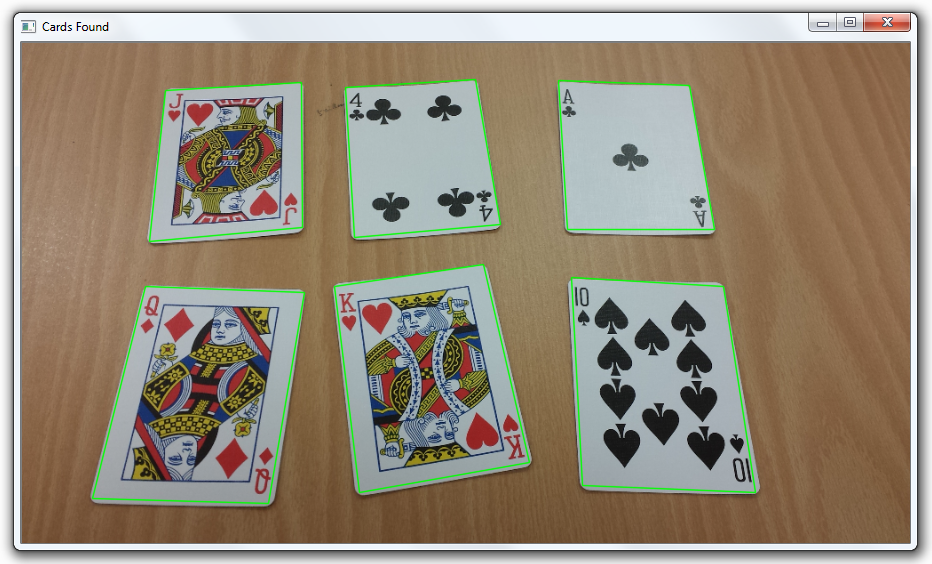
\includegraphics[width=0.6\textwidth]{chris/image1}
				\caption{}
			\end{subfigure}
		\end{figure}
		\begin{figure}[H]
			\ContinuedFloat
			\centering
			\begin{subfigure}[b]{\textwidth}
				\centering
				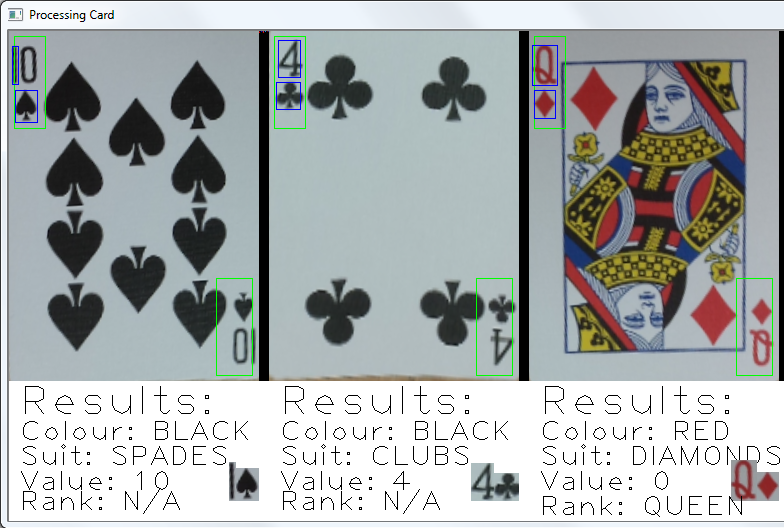
\includegraphics[width=0.6\textwidth]{chris/image2}
				\caption{}
			\end{subfigure}
		\end{figure}
		\begin{figure}[H]
			\ContinuedFloat
			\centering
			\begin{subfigure}[b]{\textwidth}
				\centering
				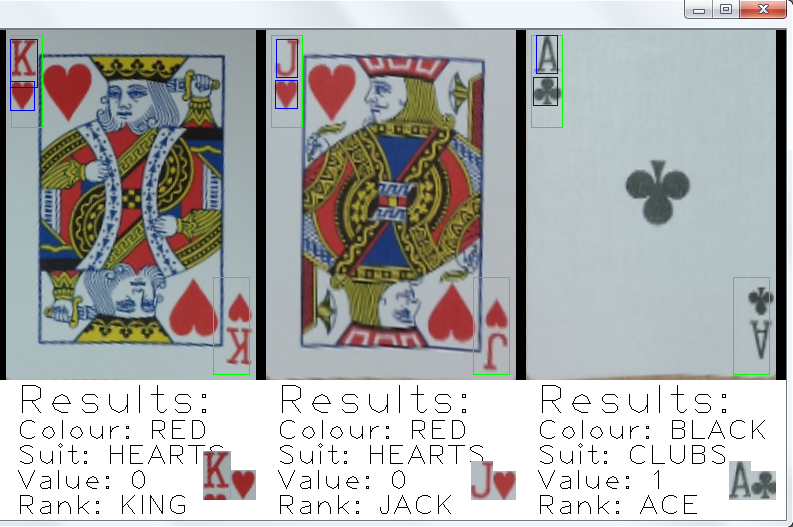
\includegraphics[width=0.6\textwidth]{chris/image3}
				\caption{}
			\end{subfigure}
			\caption{A set of playing cards (a) at various orientations with a visual output of successful classifications (b) (c)}
			\label{fig:success}
		\end{figure}

		However, when the input image is of low quality or there are too many cards per image (\textgreater $\approx$12) the classification is not always successful, but it has been found that in these situations is at least a small number are correctly identified, particularly if the unfavourable light varies across the image. Some examples of such situations are shown in Figure~\ref{fig:fail}:

		% TODO: Images with window borders from now on
		% TODO: Light distortion still an issue?
		\begin{figure}[H]
			\centering
			\begin{subfigure}[b]{\textwidth}
				\centering
				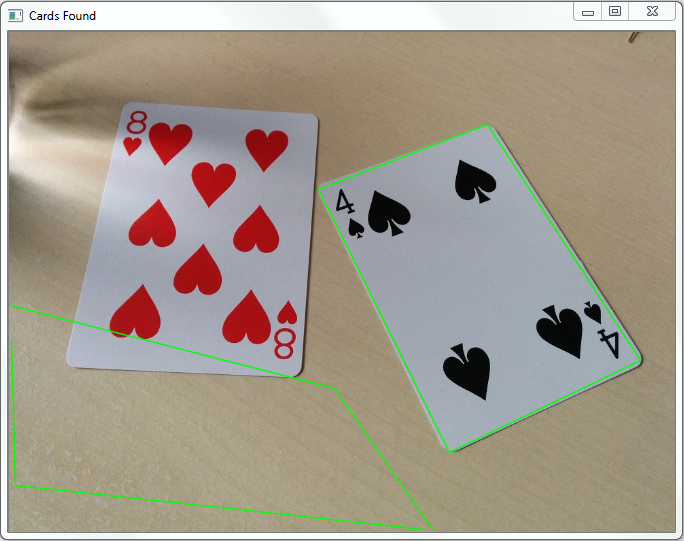
\includegraphics[width=0.6\textwidth]{chris/image4}
				\caption{}
			\end{subfigure}
		\end{figure}
		\begin{figure}[H]
			\ContinuedFloat
			\centering
			\begin{subfigure}[b]{\textwidth}
				\centering
				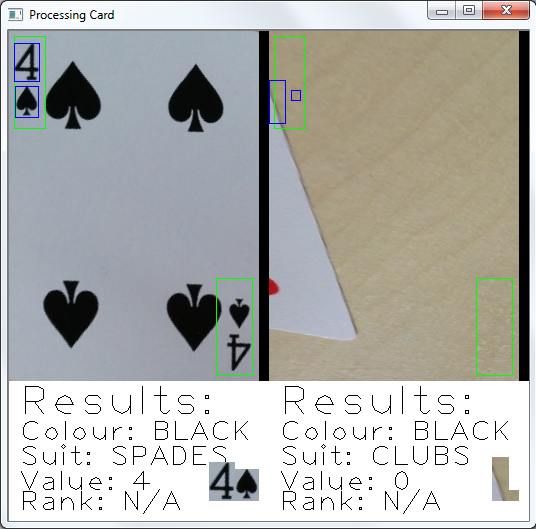
\includegraphics[width=0.6\textwidth]{chris/image5}
				\caption{}
			\end{subfigure}
			\caption{An example of miss-classification (b) due to significant lighting distortion (a)}
			\label{fig:fail}
		\end{figure}
	\counterwithin{figure}{subsubsection}

\pagebreak
\section{Review}
	\label{sec:review}
	\subsection{Review of Potential Methods}
		\subsubsection{High-level Isolation}
			For any realistic commercial application, the playing card recognition system would need to isolate individual playing cards from an input image for later classification. To do this, there exist a number of well known computer vision techniques and algorithms.

			Short of using a Haar classifier blanker solution, the technique most people would reflexively turn to is the Hough Transform \autocite{duda1972use} to detect card edges. Practically, this would be combined with generic edge detection algorithms such as Canny Edge Detection \autocite{canny1986computational}.

			% TODO: Define hysteresis
			Canny Edge Detection is particularly useful for increasing contrast and removing image noise; a process that would no doubt come in handy for isolating playing cards. A precursor to Canny Edge Detection is to blur the input image (converted to greyscale of course). This has the effect of removing specular noise. Then, areas of the image where the intensity changes with a steep gradient are marked. From these, only local maxima are preserved. A double threshold is then applied to the intensities of these local maxima that results in an image with strong and weak edges alike. Finally all edges that are not 8-connected to strong edge blobs are removed by hysteresis.

			% TODO: List parameters
			Indeed, applying Canny Edge Detection to an image of a playing card is not novel and seems to have good results. Figure~\ref{fig:cannyimg} depicts an example of doing so on a test image.

			\begin{figure}[H]
				\centering
				\begin{subfigure}[b]{0.6\textwidth}
					\centering
					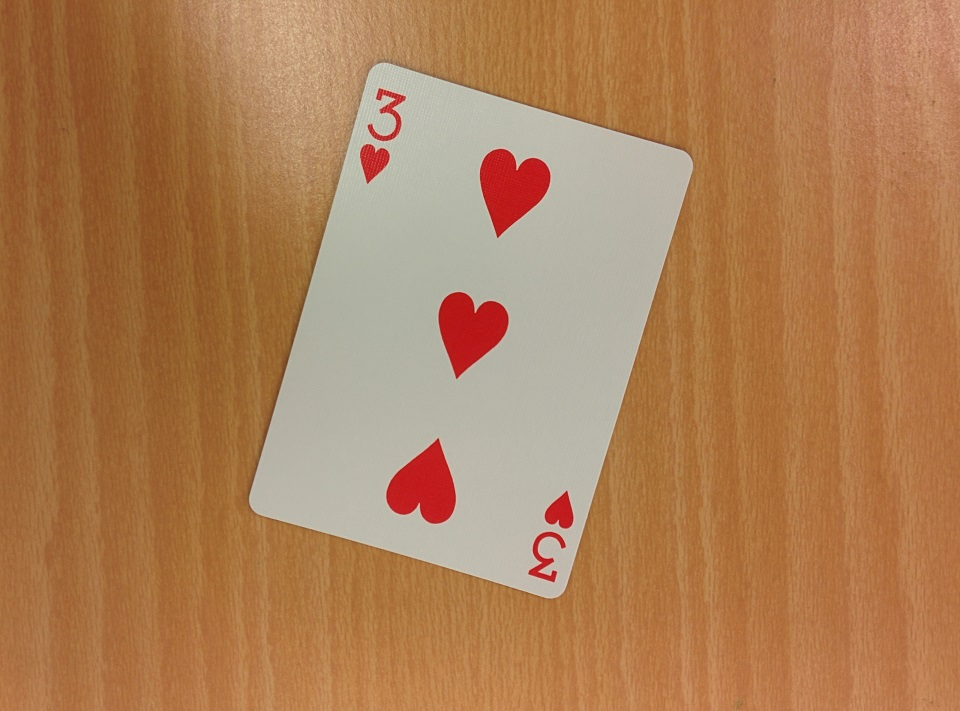
\includegraphics[width=\textwidth]{numtopred}
					\caption{}
				\end{subfigure}
			\end{figure}
			\begin{figure}[H]
				\ContinuedFloat
				\centering
				\begin{subfigure}[b]{0.6\textwidth}
					\centering
					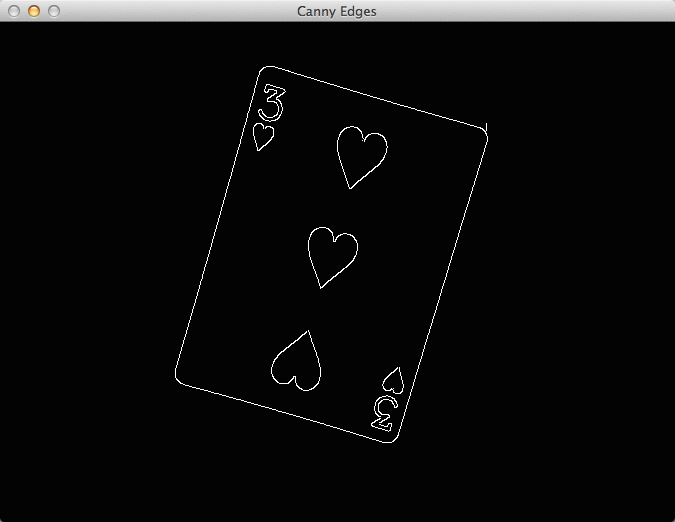
\includegraphics[width=\textwidth]{canny}
					\caption{}
				\end{subfigure}
				\caption{An example of Canny edge detection (b) as applied to test image (a)}
				\label{fig:cannyimg}
			\end{figure}

			Now that the image is binary and the edges within distinct, using the Hough Transform to extract card edges is trivial. Edges within the card are not in the shape of lines and so only a card's edges would be detected.

			The Hough Transform works in an ingenious manner; in a nutshell, each white pixel in the binary image is treated as a data point. For each of these pixels, a number of lines are drawn through them at differing angles. Then for each line at a different angle, the perpendicular distance to the origin is measured. This is then plotted in a ``Hough space'' graph. The points of intersection denote a line that intersects many points in the original image. 

			\begin{figure}[H]
				\centering
				\begin{subfigure}[b]{0.55\textwidth}
					\centering
					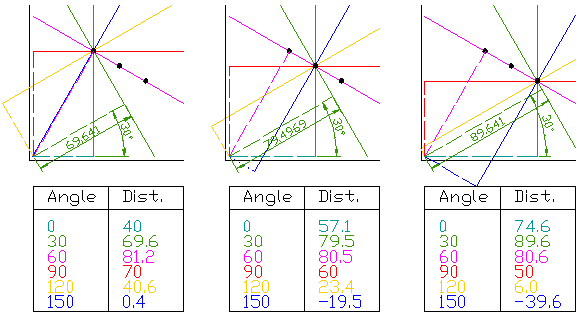
\includegraphics[width=\textwidth]{hough1}
					\caption{}
				\end{subfigure}
				\begin{subfigure}[b]{0.4\textwidth}
					\centering
					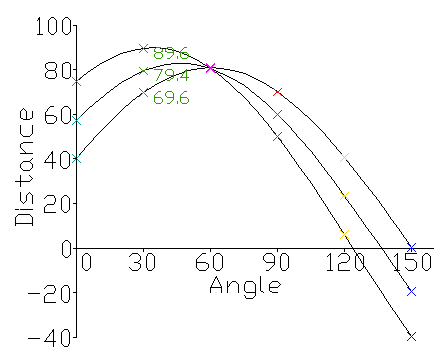
\includegraphics[width=\textwidth]{hough2}
					\caption{}
				\end{subfigure}
				\caption{The first step of the Hough transform (a) and a Hough-space graph (b); \autocite{wiki}}
				\label{fig:houghmath}
			\end{figure}

			Intuitively, one can tell how this approach can also be expanded to curves and other shapes. In practice, the Hough transform is done at a higher angular resolution and the results are stored in a matrix where cell values correspond to the number of points a line at a given angle (columns are angle and rows are distance) intersect with. The pink point in Figure~\ref{fig:houghmath} would be a cell with the value 3. This matrix would then be normalised to 255, if it was to be displayed, or not in which case the brightest points are the lines that intersect with the most points, or in this case, line up with the straightest edges. It becomes only a matter of selecting the ``brightest'' lines, or the ones that match the straightest edges. In the playing card scenario this would be the top four lines for one card. The results of this being tested can be seen in Figure~\ref{fig:hough}.

			\begin{figure}[H]
				\centering
				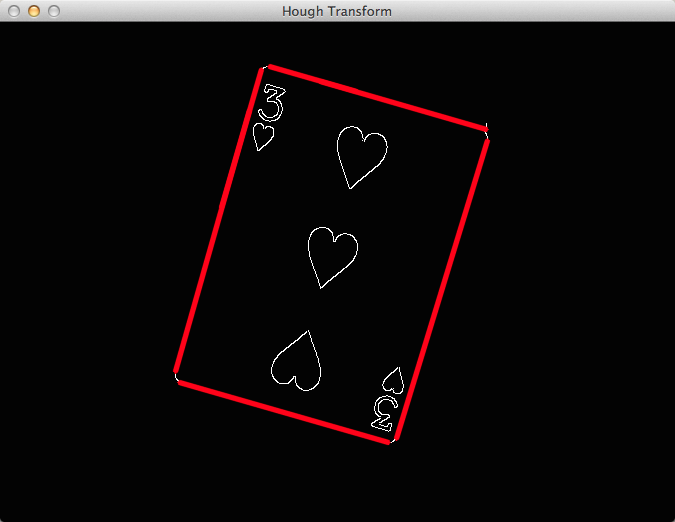
\includegraphics[width=0.6\textwidth]{hough}
				\caption{The results of a Hough transform on the Canny edges in Figure~\ref{fig:cannyimg}}
				\label{fig:hough}
			\end{figure}

			There are a number of limitations this method poses however to this application in particular. First of all, one would obviously have to programmatically calculate the points of intersection for all the four lines that the hough transform detected; the point of intersection would be a card's four corners, which can be used to construct the quadrilateral shape for subsequent perspective transformation.

			However, what if there is more than one card in the image? How would the system know how many lines to pick out and which card they belong to? If it is a question of Hough-space thresholding and distance measures for determining which lines belong to which card, then what would happen if a window was included in the image, or anything with edges and lines for that matter? Simply using the Hough transform may not be the most expandable solution for this purpose. These same limitations apply with corner detection algorithms.

			~\\

			Instead, a much more promising technique is that of finding contours through border following \autocite{suzuki1985topological}. Once a preprocessed binary image is constructed of the card input image, the darker areas around the image edges will have been thresholded out. To get around differing lighting conditions, the contours can be found for multiple binary threshold levels and compared. One problem --- as is discussed later in further detail \secref{sec:isolation} --- would be if the image itself has inconsistent lighting in different parts, such as specular reflection on a corner of the card, but a matte ambient lighting on the opposite corner.

			To get around this Contrast Limited Adaptive Histogram Equalisation (CLAHE) \autocite{pizer1987adaptive} can be utilised. This differs from standard Adaptive Histogram Equalisation (AHE) from the fact that the contrast limiting process prevents noise from being over-amplified locally within any given window as is often characteristic with standard AHE. To do this, the top of a neighbourhood's histogram is clipped at a threshold and redistributed uniformly among the histogram bins.

			It is similar in the fact that instead of equalising an entire image and simply stretching its histogram out, the image is tiled into windows that each have histogram equalisation applied to them locally. This has the effect --- as will become evident in later sections of this report --- that bright areas of the image do not become washed out and darker areas darkened out. At the same time the noise amplification issue is solved through contrast limiting.

			After binary thresholding, the card contours can be detected. One way of doing this is by computing the convex hull. A faster way is border following (by recursively visiting neighbour pixels that are on an edge) complimented by iteratively approximating a polygon within the computed polygon that has less vertices given a minimum precision. One well known technique for doing this (reducing the vertices in a polygon but still keeping it relatively similar to the original polygon) is the Ramer–Douglas–Peucker algorithm \autocite{ramer1972iterative}, \autocite{douglas1973algorithms}.

			This algorithm, expressed in plain English, works as follows. Given a curve made up of multiple points, you begin on the end points and draw a line between them. Then, you find the point that is furthest away from that line. That becomes the new edge point and the process is repeated for that curve segment. This continues until you are left with a line segment with only three points. The middle point is removed, simplifying the curve. This is done recursively until all line segments have had the same process applied to them. The result is that the final curve is simpler but still similar to the original curve. In the case of playing cards, this process would be applied to the card contours until the contour polygon only has four sides left. This polygon, or quadrilateral rather, is the shape that bounds the playing card image.

			Any of this would however need to be coupled with additional checks and custom filtration algorithms that are discussed in detail later \secref{sec:isolation}.

			~\\

			Once the contour quad is computed, the next step would be to apply a perspective transform to the area of the image that that quad encloses. Unlike an affine transform, which can apply translation, rotation, scale, and skew/shear, the perspective transform can also apply depth. In other words, a square can be turned into a trapezoid with a perspective transform while an affine can only turn it into a parallelogram.

			The perspective transform is used extensively in computer graphics to project 3D graphics onto the 2D screen plane. This gives a scene depth where things get smaller the further away they are, projected from a single point of projection, unlike an orthographic projection were things are projected along parallel lines.

			A simple example would be for instance projecting an image on the plane $z = 4$ (assume a right-handed coordinate system where the z-axis points outwards). If the point of projection is at the origin, then intuitively one expects the projection onto that plane for points where $z > 4$ that line up relative to the origin to project onto the same point. In order to operate with projective geometry, homogeneous coordinates must be used; a dimension up from affine. The perspective transformation can be expressed as:

			\begin{equation}
				P =
				\begin{bmatrix}
					1 & 0 & 0 & 0\\
					0 & 1 & 0 & 0\\
					0 & 0 & 1 & 0\\
					0 & 0 & 1 & 0
				\end{bmatrix}\qquad,\qquad
				\begin{bmatrix}
					x_c\\
					y_c\\
					z_c\\
					w_c
				\end{bmatrix}
				= P
				\begin{bmatrix}
					x\\
					y\\
					z\\
					w
				\end{bmatrix}
			\end{equation}

			where P is the perspective matrix that projects to the plane $z = 1$. However, in order make sure that the homogeneous component $w$ is equal to 1 to map back to the real plane, $(x_c, y_c, z_c)$ must additionally be divided by $w_c$; a so called perspective divide.

			Indeed, if $(x_1, y_1, z_1, w_1) = (2, 2, 2, 1)$ and $(x_2, y_2, z_2, w_2) = (4, 4, 4, 1)$ were to be projected onto $z = 1$, the result of the above transformation would give $(x'_1, y'_1, z'_1) = (1, 1, 1)$ and $(x'_2, y'_2, z'_2) = (1, 1, 1)$ which makes perfect sense intuitively, as the first point occludes the second from the perspective of the origin as projected onto $z = 1$.

			The perspective transform is crucial for deforming a pixel grid as enclosed by an arbitrary quadrilateral into a rectangle. Of course perspective transformation matrices can include any manner of transformations to project onto any plane, yet the result can always be a straightened card image matrix.
		\subsubsection{Low-level Classification}
			Once a card has been identified in the input image, its perspective transformed and isolated to a separate image, it must be classified according to suit and rank. In order to do this, techniques are available from the field of Mathematical Morphology that allow the modification of an image to enhance areas of interest as a form of pre-processing.

			In practice, these operators are implemented by passing a small group of pixels called a structuring element (SE) over the entirety of an input image, and a set of rules applied to the pixels present in the SE at each location in the image. Once the SE has been passed over the entire image, the operation is complete.

			The basic morphological operators available include \autocite{sonka1999image1}:

			\begin{itemize}
				\item Erosion --- For each image location, the output pixel is set to the lowest value within the SE.
				\item Dilation --- As for erosion, but the output becomes the highest neighbouring value. 
				\item Opening --- Combination of erosion followed by dilation. The result is an image with small areas of the foreground removed. Areas that completely house the SE are left untouched.
				\item Closing --- Similar to opening except areas smaller than the SE are filled in to the foreground.
			\end{itemize}

			All these operators can be defined mathematically using set theory. For an image matrix $X$ iterated over by a structuring element $B$, the result $Y$ of the dilation operation is the \emph{supremum}(greatest value) of the pixels in the input image under $B$ at pixel position $x$ in $X$.

			\begin{equation}
				X \oplus B = \{ Y \colon y = \sup⁡[B(x)], x \in X \}
			\end{equation}

			Similarly for erosion:

			\begin{equation}
				X \ominus B = \{ Y \colon y = \inf[B(x)], x \in X \}
			\end{equation}

			These two basic operators are then combined to produce the opening and closing operators, shown in the same terms below as the dilation of an erosion with the same sized structuring element \autocite{sonka1999image2}:

			\begin{equation}
				X \circ B = ( X \ominus B ) \oplus B
			\end{equation}

			Similarly for closing; the erosion of a dilated image:

			\begin{equation}
				X \bullet B = ( X \oplus B ) \ominus B
			\end{equation}

			Examples of the behaviour of these operators are shown in Figure~\ref{fig:morph} below:

			\begin{figure}[H]
				\centering
				\begin{subfigure}[b]{0.4\textwidth}
					\centering
					
\includegraphics[width=\textwidth]{chris/image6}
					\caption{}
				\end{subfigure}
				\begin{subfigure}[b]{0.4\textwidth}
					\centering
					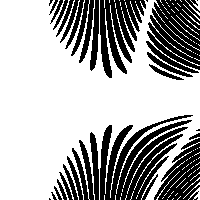
\includegraphics[width=\textwidth]{chris/image7}
					\caption{}
				\end{subfigure}\\
				\begin{subfigure}[b]{0.4\textwidth}
					\centering
					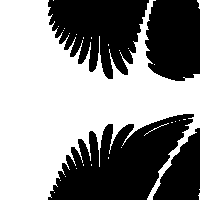
\includegraphics[width=\textwidth]{chris/image8}
					\caption{}
				\end{subfigure}
				\begin{subfigure}[b]{0.4\textwidth}
					\centering
					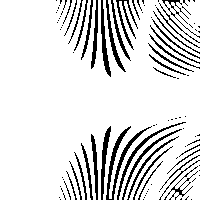
\includegraphics[width=\textwidth]{chris/image9}
					\caption{}
				\end{subfigure}\\
				\begin{subfigure}[b]{0.4\textwidth}
					\centering
					
\includegraphics[width=\textwidth]{chris/image10}
					\caption{}
				\end{subfigure}
				\begin{subfigure}[b]{0.4\textwidth}
					\centering
					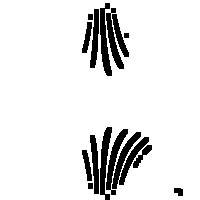
\includegraphics[width=\textwidth]{chris/image11}
					\caption{}
				\end{subfigure}
				\caption{An original image (a), after binary threshold (b). Further results of erosion (c), dilation (d), opening (e) and closing (f)}
				\label{fig:morph}
			\end{figure}

			These operators can be used to help clean up a segmented image and remove noise and spurious pixels to aid later stages of processing.
		\subsubsection{Hit-or-Miss Transform}
			The Hit-or-Miss Transform is another morphological technique that is useful as a form of binary pattern matching. This means it can be used to find instances of a desired feature image in a given sample image. In the context of classifying playing cards, this technique has potential to be used to enable the detection of the card's suit symbol as well as the rank symbol when compared to clean templates of each symbol type.

			The basis of the operation is similar to the previous operators except that the structuring element passed over the input image is that of the pattern to be found. The structuring element is divided into two sets; the `hit' set and the `miss' set. When both sets are eroded, the result is an output point wherever the input image matches the structuring element. A mathematical description of the operation is shown below, and describes the result of the Transform to be the intersection of the hit and miss sets eroded by the image $A$ and image complement $A^C$ respectively \autocite{badea}:

			\begin{equation}
				X \otimes B = ( A \ominus C ) \cap ( A^C \ominus D )
			\end{equation}

			An example of the Hit-or-Miss Transform is shown below in Figure~\ref{fig:hom}:

			\begin{figure}[H]
				\centering
				\begin{subfigure}[b]{0.3\textwidth}
					\centering
					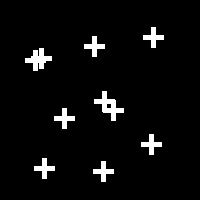
\includegraphics[width=\textwidth]{chris/image12}
					\caption{}
				\end{subfigure}
				\begin{subfigure}[b]{0.3\textwidth}
					\centering
					
\includegraphics[]{chris/image13}
					\caption{}
				\end{subfigure}
				\begin{subfigure}[b]{0.3\textwidth}
					\centering
					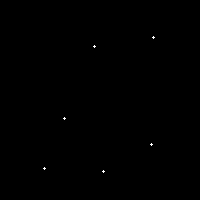
\includegraphics[width=\textwidth]{chris/image14}
					\caption{}
				\end{subfigure}\\
				\begin{subfigure}[b]{0.3\textwidth}
					\centering
					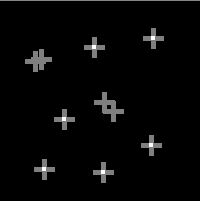
\includegraphics[width=\textwidth]{chris/image15}
					\caption{}
				\end{subfigure}
				\caption{A sample image of symbols (a) processed with a structuring element (b) yields markers wherever there is a match (c). Overlaid on input image with large markers (d).}
				\label{fig:hom}
			\end{figure}

			Note in the above figure that no markers are present when the SE symbol is obstructed. This prevents a complete match. In this way it is possible to locate a pre-determined symbol inside a larger image by iterating over the entire matrix.
\pagebreak
\section{Proposed Method}
	\counterwithin{figure}{subsection}
	\subsection{Sub-task Breakdown}
		After review of the applicable processing methods in the previous section, the initial task list from Section~\ref{sec:task} can be expanded in more detail. Figure~\ref{fig:flowchart} shows the techniques used at each stage and the resulting classification information obtained:

		\begin{figure}[H]
			\centering
			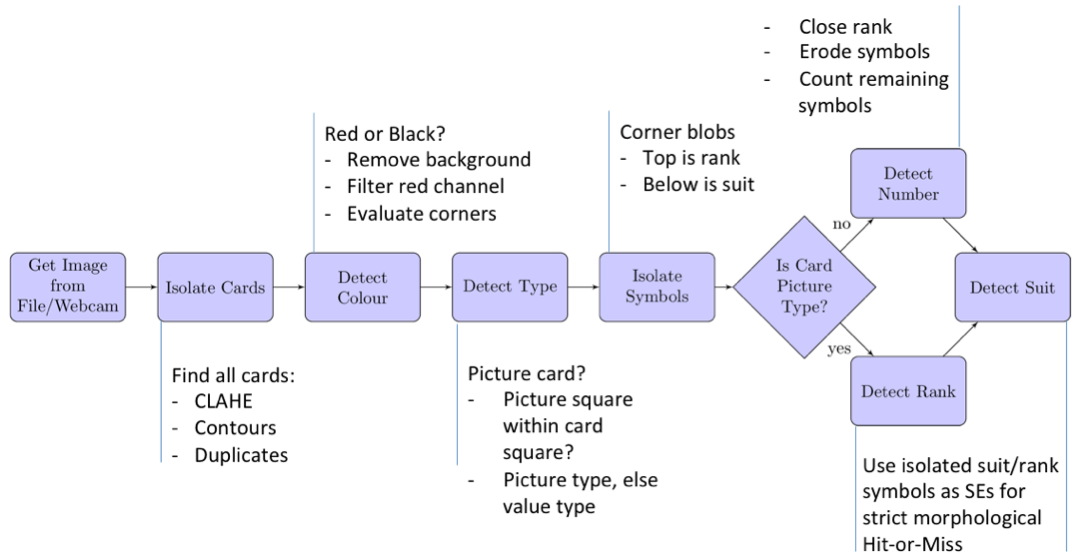
\includegraphics[width=\textwidth]{chris/flowchart}
			\caption{Sub-task flowchart showing processing stages and methods used for each}
			\label{fig:flowchart}
		\end{figure}

		\begin{itemize}
			\item The first stage is to load the input image, from either a local directory or captured from a connected webcam. 
			\item Once this is done the individual cards must be extracted from the input image to separate images for later classification. This will be done by using Contrast Limited Histogram Equalisation to compensate for varying illumination and contour detection to locate the card parallelograms. Finally the locations of the contours will be compared to discard duplicates that are too close to each other e.g.: multiple contours for one card as a result of shadows.
			\item The next stage is to detect the suit colour of the card. This will be used to reduce the search space of the suit itself. For example, a red suit can only logically be a diamonds or hearts card. This helps reduce confusion between the two at a later processing stage. This will be achieved by removing the white background and evaluating the red surface area within the two rank and symbol corners. Above a threshold and the suit must be a red one.
			\item Next the type of the card is determined; a value card (2 to 10) or a picture card (Jack, Queen, King). An Ace is a value one card. If an isolated card image contains a contour within it, it must be a picture card as the inner contour contains the illustration. 
			\item The suit symbol and rank symbol must be isolated as sub-regions to be used later for isolation. This is done by isolating the corner containing the symbols and searching for blobs from the top. The first encountered will be the rank, and the second below it will be the suit symbol.
			\item Depending on the result of the Detect Type stage, the card is classified differently depending on its type.  If it is a picture card, the rank symbol is pattern matched against a pre-created template for each of the `J', `Q' and `K' rank symbols and the strongest match will be the rank of that card. However, if the card is a number card, it is classified in a different manner. This will involve removing the suit and value symbol and using the erosion and closing morphological operations to reduce the remaining suit symbols to a number of countable blobs equal to the value of the card. 
			\item The final stage of classification is to determine the actual suit of the card. This is done in a similar fashion to determining the rank of a picture card as previously discussed, except the pre-created templates are those of each of the suits; diamonds, clubs, hearts and spades.
		\end{itemize}
	\counterwithin{figure}{subsubsection}
\pagebreak
\section{Implementation}
	\label{sec:implementation}
	% Program flow
	\subsection{Image IO/Webcam IO}
				The loading of images to analyse from either disk or webcam is one of the most basic uses of the OpenCV library. To load in image from a file on a local or network hard disk drive, the \code{cv::imread()} function is called with the path to the image and read mode supplied as arguments. This is shown in the code segment below for an image path supplied as the second command line argument to be read as a colour image:

		\begin{lstlisting}

cv::Mat input = cv::imread(argv[1], CV_LOAD_IMAGE_COLOR);
		\end{lstlisting}

		Once this call has been made, the image matrix is checked for integrity by examining the width and height of the \code{cv::Mat} returned from \code{cv::imread()}:

		\begin{lstlisting}

cv::Size input_size = input.size();

//Check size is greater than zero
if(input_size.width > 0 && input_size.height > 0)
{
	...
}
		\end{lstlisting}

		If this check succeeds, the image is valid and is passed on to \code{process_image()} for further processing and eventual classification. Otherwise the program terminates with a suitable error message:
		
		\begin{lstlisting}

if (process_image(input))
	return EXIT_FAILURE;
		\end{lstlisting}

		If the `--cam' command line argument is supplied, the image is instead loaded from a webcam frame during live capture. A loop is entered displaying images from the webcam until the space bar is pressed, the loop is exited and the image processed as shown previously. This decision process is shown below:

		\begin{lstlisting}

bool from_cam = !strcmp(argv[1], "--cam");

...
//Open a webcam source
cv::VideoCapture cap(CV_CAP_ANY);
cv::waitKey(1000);

if(!cap.isOpened())
{
	cerr << "Unable to access webcam" << endl;
	return -3;  //Incorrect arguments code
}

cout << "Press space to take a photo" << endl;

char key;
do
{
	key = cvWaitKey(10);

	cap >> input;

	cv::imshow("Webcam", input);

	// Break out of loop if Space key is pressed
} while (char(key) != 32);
		\end{lstlisting}

		Once the isolation and classification of any cards present in the captured webcam frame is complete, the user can opt to capture another frame or exit the program.
	\subsection{Card Data Structure}
		After loading an image, the intermediary and final results of isolation and classification are stored in a data structure to adequately separate all the data for each real card as an equivalent \verb!C++! object. This is the Card class:

\begin{lstlisting}

class Card {
public:
\end{lstlisting}

\begin{itemize}
    \item Enumerations for the Suit, PictureRank and Colour attributes:
\end{itemize}

\begin{lstlisting}
	//Suit enumeration
	enum Suit {
	    CLUBS,
	    DIAMONDS,
	    HEARTS,
	    SPADES,
	    UNKNOWN_SUIT
	};

	//Picture card rank enumeration
	enum PictureRank {
	    RANK_JACK,
	    RANK_QUEEN,
	    RANK_KING,
	    RANK_ACE,
	    UNKNOWN_RANK
	};

	//Suit colour enumeration
	enum Colour {
	    BLACK,
	    RED,
	    UNKNOWN_COLOUR
	};
\end{lstlisting}

\begin{itemize}
    \item Configuration data for the final dimensions of the isolated card, the regions to be considered as the corners and GUI output colours:
\end{itemize}

\begin{lstlisting}
	static const int WIDTH = 250, HEIGHT = 350, AREA = 250*350, CORNER_AREA;
	static const cv::Rect TOP_CORNER_RECT;
	static const cv::Rect BOTTOM_CORNER_RECT;
	static const cv::Scalar LINE_COLOUR, LINE_COLOUR_ALT;
	static const cv::Scalar TEXT_COLOUR;
\end{lstlisting}

\begin{itemize}
	\item Data storage for intermediate \code{cv::Mat} objects used for classification as well as the object attributes that store the actual classification results themselves:
\end{itemize}

\begin{lstlisting}
	//Data
	cv::Mat mat, mat_clahe, mat_bin, mat_sym, mat_rank;
	Suit detected_suit;
	Colour detected_colour;
	PictureRank detected_rank;
	int detected_value;
	bool is_picture_card;
	cv::Rect _last_aabb, _rank_aabb;
\end{lstlisting}

\begin{itemize}
	\item Constructor and function prototypes for manipulation of the object within the larger scope of the program:
\end{itemize}

\begin{lstlisting}
	//Constructor declarations
	Card();
	Card(cv::Mat);

	//Functions
	void set_mat(cv::Mat mat);
	void init();
	void show();
	void show_with_card(cv::Mat card);
	cv::Mat results_to_mat();
	cv::Mat as_mat_with_results();
};
\end{lstlisting}

Using this object orientated approach to data storage simplifies the tasks of keeping track of isolated cv::Mats and classified attributes for each card in the input image, and also allows iteration through all cards in a \code{std::vector}. Most importantly it allows calling any of the classification functions such as \code{void detect_value_picture(Card *card)} by passing a pointer to the object and guaranteeing that the required member (for example \code{Card::mat_rank} for the isolated rank image matrix) is available for use within that function.

The usefulness of this capability is shown by the high level of abstraction possible in the main part of the software as shown below:

\begin{lstlisting}

for(size_t i = 0; i < cards.size(); i++)
{
    Card *card = &cards[i];

    //Detect suit colour
    detect_colour(card);

    //Detect suit type (number/picture)
    detect_type(card);

    //Find symbols
    find_symbols(card);

    //Get card value
    if (!card->is_picture_card)
    {
        detect_value_number(card);
    }
    else
    {
        detect_value_picture(card);
    }

    //Find suit
    find_suit_sym(card);
}

//Show results until key press
show_cascade(cards);
\end{lstlisting}
	\subsection{Card Isolation}
		\label{sec:isolation}
		Once an image is passed in as an input, the first step is to find one or more cards in the image and, if any were found, extract them from the image and prepare them for processing. This is done in a number of steps.

		\subsubsection{Card Detection}
			In order to detect cards within the image, the function \code{find_cards()} in \source{isolation.cpp}{app:isolationcpp} is called from \source{main.cpp}{app:maincpp}. It takes in an empty \code{std::vector} of objects of type \code{Card} as an inputs which it then populates with the detected cards for later processing.

			Cards are detected by finding quadrilaterals with a method not unlike the one used in the sample file \emph{squares.cpp} in the official OpenCV repository \autocite{squares} albeit with some decisive distinctions. The backbone of the algorithm is the OpenCV function \code{cv::findContours()}. This function retrieves contours from a binary image using the algorithm developed by \textcite{suzuki1985topological} via border following. It was decided not to implement a custom function since it would not have added any flexibility or speed advantage over the OpenCV implementation. Indeed it would only have increased code complexity.

			This function requires a binary image as an input. As such, input images undergo a series of processing stages beforehand. First, they are converted to greyscale. Then CLAHE --- as explained previously \secref{sec:isolation} --- is applied to these images. The size of the CLAHE window varies between 32x32 and 28x28 pixels depending on if the user has specified with the \code{--multi} command line flag that the program should run in multiple card mode. CLAHE operations using OpenCV functions run on the GPU through CUDA; they cannot be optimised by writing custom code for CLAHE without utilising CUDA, which would only introduce system-level bugs that have been long since resolved within OpenCV's code base. For this reason, the OpenCV CLAHE implementation was used. Figure~\ref{fig:clahe} shows a side by side comparison of normal HE and CLAHE on an image of a playing card that has a bright top-right corner:

			\begin{figure}[H]
				\centering
				\begin{subfigure}[b]{0.5\textwidth}
					\centering
					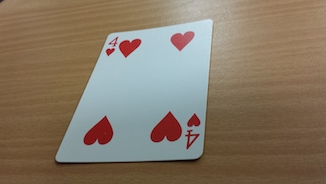
\includegraphics[width=\textwidth]{pers2}
					\caption{}
				\end{subfigure}
			\end{figure}
			\begin{figure}[H]
				\ContinuedFloat
				\centering
				\begin{subfigure}[b]{0.4\textwidth}
					\centering
					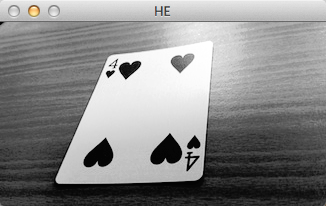
\includegraphics[width=\textwidth]{he}
					\caption{}
				\end{subfigure}
				\qquad
				\begin{subfigure}[b]{0.4\textwidth}
					\centering
					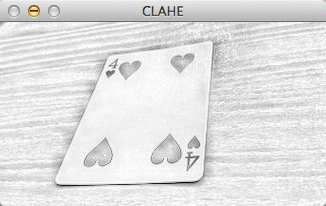
\includegraphics[width=\textwidth]{clahe}
					\caption{}
				\end{subfigure}
				\caption{HE (b) and CLAHE (c) as applied to a test image (a)}
				\label{fig:clahe}
			\end{figure}

			After performing CLAHE, the image is blurred. The amount of blur is set as a function of it image's dimensions. More specifically \code{(image_size.width + image_size.height) >> 8} or in plain English, the perimeter of the image divided by 512. This prevents small images from losing too much detail through blurring while large images do not remain too sharp. Blurring is done to filter out noise for the next step.

			The resulting image is then converted to binary using the threshold parameter before \code{cv::findContours()} is called. Contours are found for processed binary images for thresholds ranging from 150 to 255 (both inclusive) in increments of 2. This bright range was experimentally determined to be the best to create binary images from. Figure~\ref{fig:clahebin} show an example of binary thresholding at only one value (210) on the pure HE image, and the CLAHE image.

			\begin{figure}[H]
				\centering
				\begin{subfigure}[b]{0.4\textwidth}
					\centering
					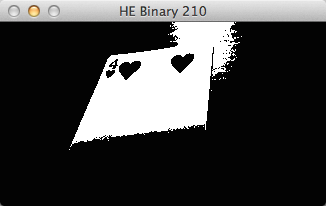
\includegraphics[width=\textwidth]{hebin}
					\caption{}
				\end{subfigure}
				\qquad
				\begin{subfigure}[b]{0.4\textwidth}
					\centering
					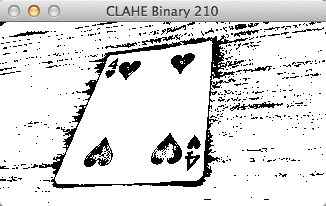
\includegraphics[width=\textwidth]{clahebin}
					\caption{}
				\end{subfigure}
				\caption{Binary thresholding at 210 on the HE (a) and CLAHE (b) of the test image in Figure~\ref{fig:clahe}}
				\label{fig:clahebin}
			\end{figure}

			Notice how The HE image over-accentuates the bright spot on the top left and casts the rest of the image into darkness. The contours that would be computed for this shape would encroach onto the desk and miss the bottom half of the card entirely. Meanwhile the CLAHE image provides a nice border around the card that can be followed, has no sign of the bright spot ever existing, and leaves the rest of the blobs inconspicuous enough that they can be filtered out.

			The found contours are approximated into geometry using with the function\\\code{cv::approxPolyDP()} and then go through a number of rigorous checks. Contours that do not pass these checks are discarded and not added to the final contours collection that the function populates. These include:

			\begin{enumerate}
				\item Does the contour have four corners?\\[4px]
					Although card contours can have more than 4 approximated corners if the cards are bent or folded significantly, most will not, so the design does not handle card contours with more than four corners.
				\item Is its area greater than 4\% of the whole image?\\[4px]
					This is to filter out noise.
				\item Is it convex in shape like card borders?
				\item Is its area less than 75\% of the image?\\[4px]
					This is to filter out borders.
				% TODO: More detail? Including reason for fixing?
				\item Is it not inside another previously detected contour or another inside it?\\[4px]
					Calculated mathematically from vertex coordinate information. This is to filter out symbol (e.g. diamonds) and picture card misclassification. Previously detected contours in the list that turn out to be contained by newly detected contours are replaced by the newly detected and discarded.
				\item Is it significantly dissimilar to previously detected contours?\\[4px]
					The criteria for this check are that every rotation of the four contour vertices are at least a certain total distance away from their counterparts (summed up manhattan/city block distance in pixels). This minimum total distance is a function of the image size to normalise pixel units into units relative to the image dimensions. This relationship is \code{(image_size.width + image_size.height) * 0.5F * min_square_diff} or in other words, the mean image side length (to account for disproportionate image aspect ratios) multiplied by a constant factor set to $0.1$, i.e. 10\% of the mean image side length.
			\end{enumerate}

			Once all contours have been iterated through and the ones that fail these criteria have been filtered out, the result is a collection of contour quads that surround at least every card in the image (in the form of a \code{vector<vector<cv::Point>>} --- a vector of vectors with four points each). \emph{At least} every card in the image; the pruning process is not yet over!

			The assortment of contours go through a secondary, later filtration process that requires processing the pixel data within these contours. To do this --- as well as to construct the card image matrices for subsequent classification --- the contour quad data is used to perspective transform the original image into a rectangular image of the card, an operation reviewed previously \secref{sec:isolation}.

			\begin{figure}[H]
				\centering
				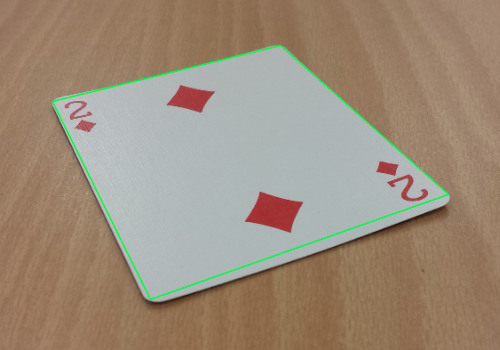
\includegraphics[width=0.6\linewidth]{perstrans1}
				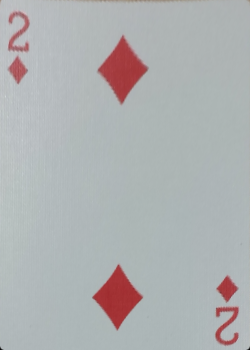
\includegraphics[width=0.3\linewidth]{perstrans2}
				\caption{Output of perspective transform of contour quad from test image}
				\label{fig:perstrans}
			\end{figure}

			The perspective transform is low-level enough that its implementations do not vary much at all. The maths involved in calculating the 3x3 matrix of a perspective transform that can be used to map pixels at a perspective to other shapes/perspectives is standard but cumbersome to implement (unlike an affine transform). For these reasons, the OpenCV function \code{cv::getPerspectiveTransform()} was used. It takes two quads as inputs and returns the map matrix. The source quad is the detected contour and the destination quad is a simple 250x350 rectangle which matches the standard 5:7 poker card aspect ratio like in figure~\ref{fig:perstrans}.

			The transformation matrix is then used in the function \code{cv::warpPerspective()} which deforms the pixel grid of the source image and maps it to the destination image while interpolating transitional pixels; a process that is both non-trivial as well as distant from the task at hand. The image matrix produced through this process is subsequently used to instantiate a new \code{Card} object.

			On instantiation, the \code{Card} constructor additionally generates an 8x8 CLAHE version and a 140 threshold binary version of the card image matrix, which are publicly accessible from a \code{Card} object. Once instantiated, the card's binary image matrix is finally used for the last phase of isolation filtering.

			The last criteria for what makes a card is its whiteness measure. The measure is simple; all non-zero (i.e. white) pixels in the card image matrix are counted and the final value is divided by the card's area giving a float that describes the proportion of whiteness in the card. The whiteness threshold is set to an experimentally practical \code{0.5F} or 50\% bearing in mind that error due to lighting inconsistency is a non-issue following CLAHE. Cards that are not white enough are discarded. This solves false detections such as that in figure~\ref{fig:whiteness}.

			\begin{figure}[H]
				\centering
				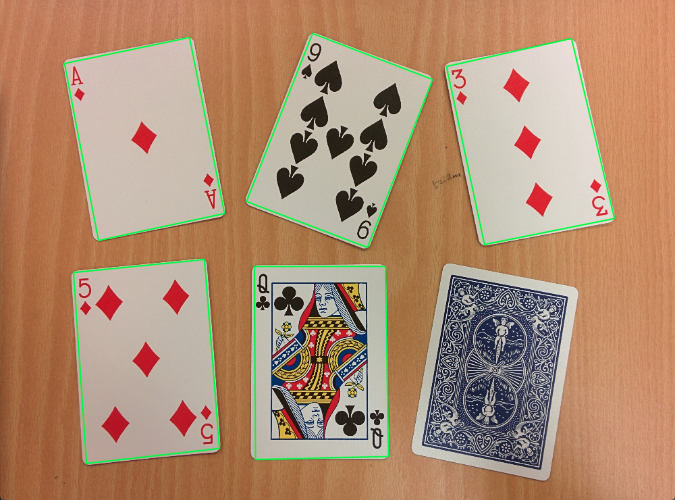
\includegraphics[width=0.9\linewidth]{whiteness}
				\caption{Example of whiteness check ignoring overturned card}
				\label{fig:whiteness}
			\end{figure}

			Finally, there is one more processing step that needs to be undertaken before a detected card is deemed worthy enough to join its brethren in the detected card vector and \code{find_cards()} can return\ldots

		\subsubsection{Rotation Correction}
			One critical issue was the problem of a sequence of contour quad vertices starting at the wrong corner and, as a direct consequence, causing the final card image matrix to be perspective transformed incorrectly. This problem became evident when processing cards where the top-most corner in the image is numbered, such as the lower examples in figure~\ref{fig:rot}; the card could just be at a very strange perspective that projects to that shape.

			\begin{figure}[H]
				\centering
				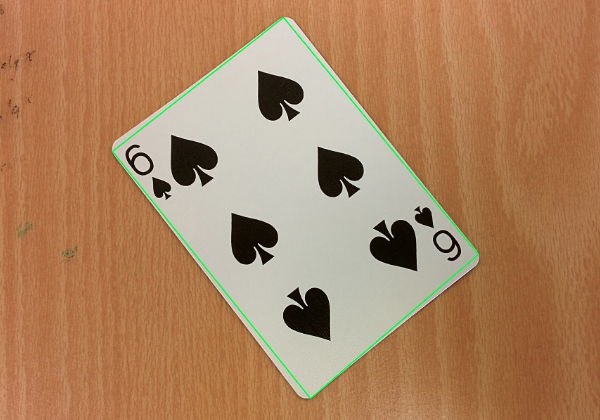
\includegraphics[width=0.6\linewidth]{rot1}
				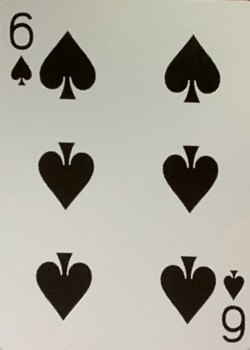
\includegraphics[width=0.3\linewidth]{rot2}\\[5px]
				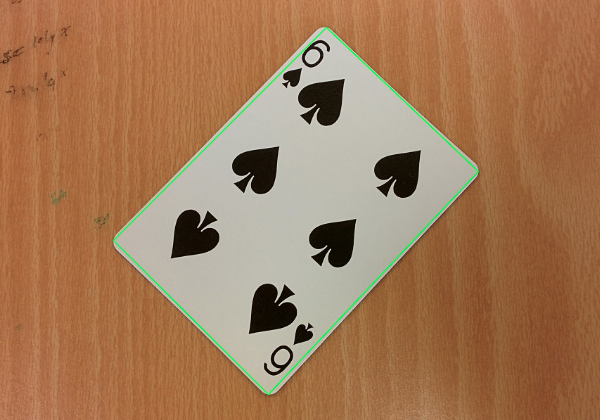
\includegraphics[width=0.6\linewidth]{rot3}
				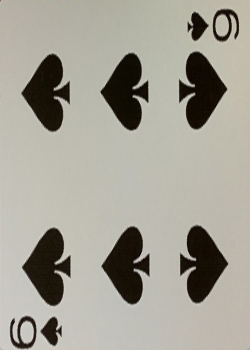
\includegraphics[width=0.3\linewidth]{rot4}
				\caption{Example of erroneous perspective transformation}
				\label{fig:rot}
			\end{figure}

			The solution developed is simple and works very well. The same measure of whiteness as is used for the whole card is applied to both the top left and the bottom right corners of the card image matrix (the bounds for which are defined as static constants in the \code{Card} class based on physical measurements). If corner whiteness surpasses 80\%, the card quad is rotated by one vertex --- the direction or rotation being arbitrary due to a card's symmetry --- and transformed into a new image matrix.

			The corner whiteness for this new image matrix is also measured, and compared against old corner whiteness. If it has a lesser corner whiteness measure than the old, that means that the old card image matrix was indeed oriented incorrectly and so the new one is used instead. If the opposite holds true, then the first overall whiteness threshold was passed incorrectly (perhaps due to some unusual specular lighting that the CLAHE did not quite catch) and so the new image matrix is discarded and the old one's usage is continued as if nothing ever happened.

			At long last, the \code{Card} vector contains all detected cards --- to a high degree of accuracy --- ready for individual processing and classification by the rest of the program, and the function can return.
	\counterwithin{figure}{subsection}
	\subsection{Colour Detection}
				The set of four traditional playing card suits are split into two further subcategories; diamonds and hearts in red, and clubs and spades in black. This information can be determined beforehand when classifying a card and used to reduce the suit symbol search space, as well as help increase detection accuracy. For example, when compared side by side, the hearts and spades suits both appear similar due to their curves and large surface area, with the spaces symbol appearing similar to a heart when viewed upside down.

		\begin{figure}[H]
			\centering
			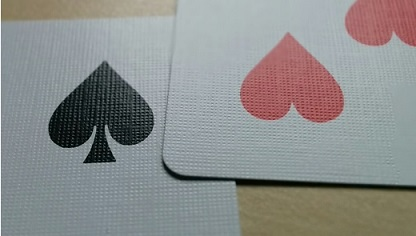
\includegraphics[width=0.6\linewidth]{chris/image16}
			\caption{Hearts and Spades can look similar, highlighting the usefulness of colour information integration.}
			\label{fig:colours}
		\end{figure}

		% TODO: Also to divide HoM search space by 2
		Using this line of thinking, the top left and bottom right corners of the card are evaluated according to their `redness'. A card that has a large surface area of `redness' is likely to be either a diamonds card or a hearts card. The first stage in this step of classification is to make the background of the card completely black. The reason behind this is that a white pixel is as bright as it is due to a large red component, along with large green and blue components also. By transforming all white pixels above a threshold into black pixels, only the majority-red pixels will remain. This is implemented as shown below:
		
		\begin{lstlisting}

//For all pixels...
for(int y = 0; y < input_size.height; y++)
{
	for(int x = 0; x < input_size.width; x++)
	{
		//Get BGR values
		int b = in_data[(y)*input.step + (x)*input_channels + 0];
		int g = in_data[(y)*input.step + (x)*input_channels + 1];
		int r = in_data[(y)*input.step + (x)*input_channels + 2];

		//Set output pixel
		if(b > white_level && g > white_level && r > white_level)
		{
			//Make it black
			out_data[(y)*output.step + (x)*output_channels + 0] = 0;
			out_data[(y)*output.step + (x)*output_channels + 1] = 0;
			out_data[(y)*output.step + (x)*output_channels + 2] = 0;
		}
		else
		{
			//Leave pixel as it is
		}
	}
}
		\end{lstlisting}

		The result of this operation is illustrated below in Figure~\ref{fig:whitebg}:
		\begin{figure}[H]
			\centering
			\begin{subfigure}[b]{0.4\textwidth}
				\centering
				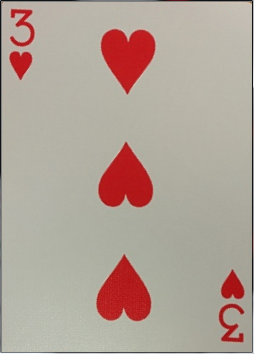
\includegraphics[width=\textwidth]{chris/image17}
				\caption{}
			\end{subfigure}
			\begin{subfigure}[b]{0.4\textwidth}
				\centering
				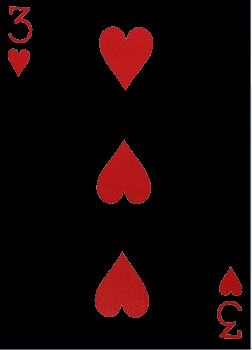
\includegraphics[width=\textwidth]{chris/image18}
				\caption{}
			\end{subfigure}
			\caption{An isolated card (a) with white background pixels removed (b).}
			\label{fig:whitebg}
		\end{figure}

		Once this is complete, the image is then filtered to remove all green and blue component values, leaving a purely red image:
		
		\begin{lstlisting}

//For all pixels...
for(int y = 0; y < input_size.height; y++)
{
	for(int x = 0; x < input_size.width; x++)
	{
		//Set output pixel              
		out_data[(y)*output.step + (x)*output_channels + 0] = new_value;    //B
		out_data[(y)*output.step + (x)*output_channels + 1] = new_value;    //G 
	}
}
		\end{lstlisting}

		where \code{new_value} is set to 0 (black). The red component is left untouched. The result is shown below:

		\begin{figure}[H]
			\centering
			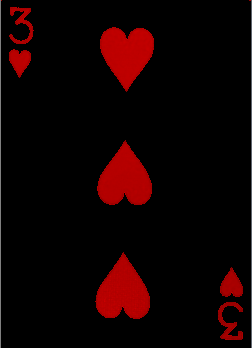
\includegraphics[width=0.4\textwidth]{chris/image19}
			\caption{An isolated card (a) with white background pixels removed (b).}
			\label{fig:redchan}
		\end{figure}

		The final step in this suit colour processing stage is to evaluate whether the top-left and bottom-right corners are sufficiently high in red surface area that they can be classified as belonging to a red suit. This final step of implementation is shown below (abbreviated):

		\begin{lstlisting}

bool is_red_suit_by_corners(cv::Mat input, int base_threshold, int target_regions, float perc_red)
{
	...

	//Get four corner regions
	int region_width = Card::TOP_CORNER_RECT.width;
	int region_height = Card::TOP_CORNER_RECT.height;

	//Create region matrices, top left, bottom right...
	cv::Mat regions[2] = {
		input(Card::TOP_CORNER_RECT),
		input(Card::BOTTOM_CORNER_RECT)
	};

	//For all regions...
	for(int i = 0; i < 2; i++)
	{
		//Reset totals
		red = 0; green = 0; blue = 0;

		//Pointer to data
		uchar *data = (uchar*)regions[i].data;

		//Get region channels once for speed
		int region_channels = regions[i].channels();

		//For all pixels...
		for(int y = 0; y < region_height; y++)
		{
			for(int x = 0; x < region_width; x++)
			{
				//Get values
				int b = data[(y)*regions[i].step + (x)*region_channels + 0];
				int g = data[(y)*regions[i].step + (x)*region_channels + 1];
				int r = data[(y)*regions[i].step + (x)*region_channels + 2];

				if(max(r, g, b) == r && r > base_threshold)
				{
					red++;
				}
				else if(max(r, g, b) == g && g > base_threshold)
				{
					green++;
				}
				else if(max(r, g, b) == b && b > base_threshold)
				{
					blue++;
				}
				else {
					//No action
				}
			}
		}

		//Compute result
		float total = (float)region_width * (float) region_height;
		float match_perc = (float) red / total;
		regions_red[i] = (red > blue && red > green) && match_perc > perc_red;
		
		...
	}

	//Count number of red regions
	int count = 0;
	for(int c = 0; c < 2; c++)
	{
		if(regions_red[c] == true)
		{
			count++;
		}
	}

	...

	return count >= target_regions;
}
		\end{lstlisting}

		Thus if both the examined regions are found to be majority red above the parametrised percentage specified, the function returns \code{true}, meaning the card suit is a red suit, either diamonds or hearts. The result structure is then assigned the appropriate colour enumeration constant.

		When called as part of card isolation, the call appears as below:

		\begin{lstlisting}

card->detected_colour = is_red_suit_by_corners(working, 100, 2, 0.10F) ? Card::RED : Card::BLACK;
		\end{lstlisting}
	\subsection{Type Detection}
		\label{sec:typedet}
		The next step is to figure out if a card is a picture or number type. This is particularly crucial for the branching down the pipeline in which picture card rank is detected with one algorithm while number card rank is detected with another \secref{sec:numdet}.

		Fortunately, with standard brand Bicycle\textregistered~poker cards --- the most common playing cards in the world --- detecting a card's type is not very difficult. Figure~\ref{fig:picture} shows an example of a picture card. Notice how the picture is completely boxed in (also refer to \ref{fig:innercont}).

		\begin{figure}[H]
			\centering
			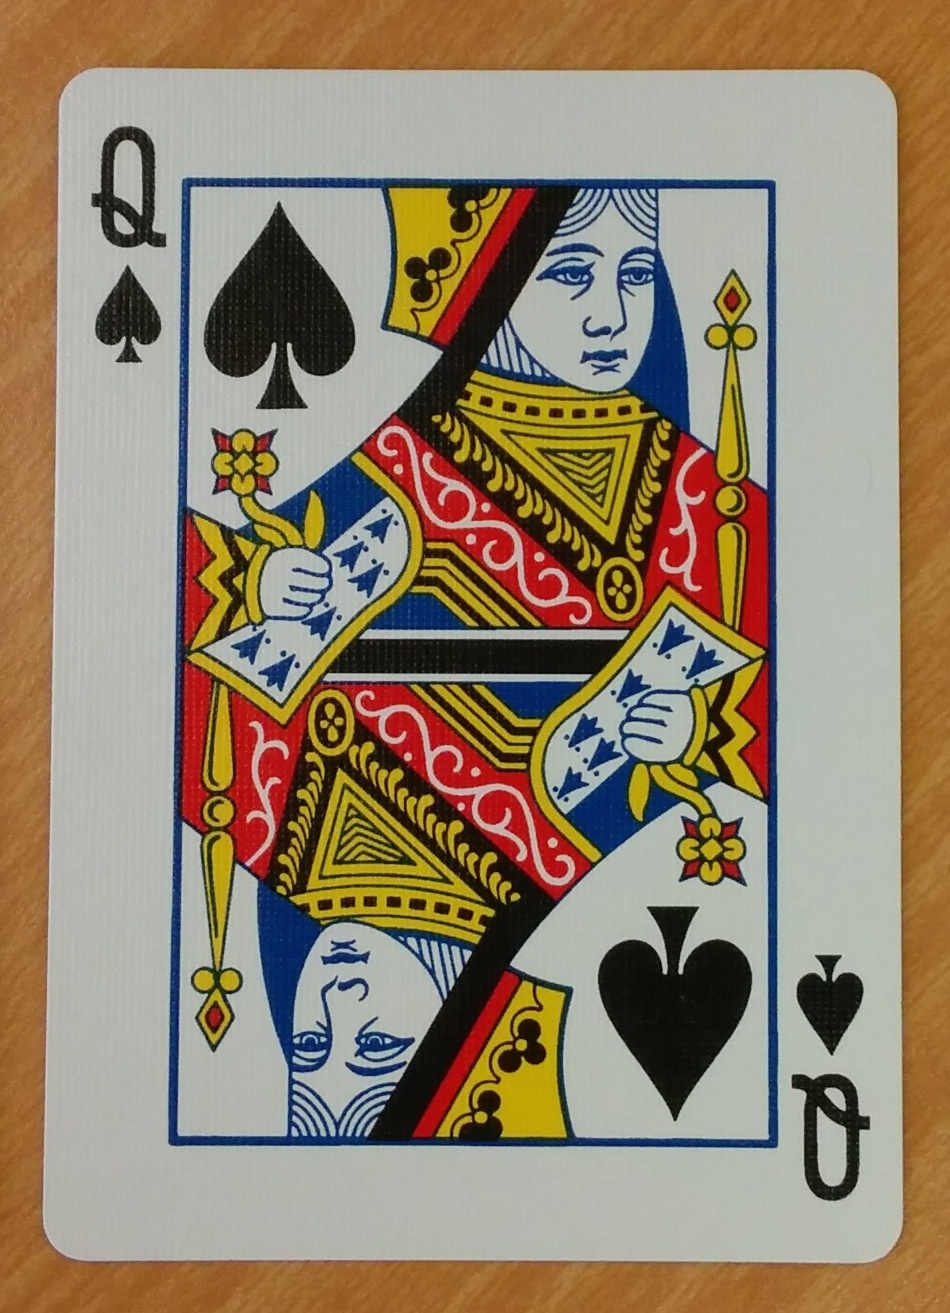
\includegraphics[width=0.4\textwidth]{picture}
			\caption{The queen of spades picture card}
			\label{fig:picture}
		\end{figure}

		The same function that was used for finding card contours earlier \secref{sec:isolation} in \source{isolation.cpp}{app:isolationcpp}, \code{find_quads()}, is also applied to a card's image matrix from within the function \code{detect_type()} in \source{classification.cpp}{app:classificationcpp}. If a single quad contour with an area large enough for it not to be the ace of diamond's diamond is found within the card, it is classified as a picture card and that information is stored the card's \code{Card} data structure.
	\subsection{Value/Rank and Suit Symbol Isolation}
		Since pure HoM was found to (unsurprisingly) be very time intensive, even after cutting the templates to be matched in half via colour detection, a shortcut needed to be found for rank and suit detection. The solution is to locate and isolate the value/rank symbol and the suit symbol and, once scaled, apply HoM to just those subimages.

		This is done in a simple yet extremely effective manner at the bottom of \source{isolation.cpp}{app:isolationcpp} starting with the function \code{find_symbols()}, which, like \code{find_cards()}, is called from \source{main.cpp}{app:maincpp}.

		The algorithm developed specifically for this purpose can be described as follows:

		\begin{enumerate}
			\item For each pixel in card's binary image matrix within the bounds of the top left corner rectangle search space (green in figure~\ref{fig:symfind}):
			\begin{enumerate}
				\item If a pixel is black, clone the card's binary image matrix and flood-fill the blob out of the original (to not repeat the operation on the same blob again).
				\item Perform an XOR crop --- with the clone, and the original card's binary image matrix with the blob flood-filled white as inputs --- to get an axis-aligned bounding box (AABB) around the detected blob.
			\end{enumerate}
			\item If a blob was found, set the card's value/rank image matrix to the first blob found (the top and leftmost).
			\item If a blob was found, set the card's suit symbol image matrix to the last blob found (the bottom and leftmost).
		\end{enumerate}

		The trick here is the XOR crop (\code{xor_crop()} in \emph{isolation.cpp}), a function written explicitly for use in \code{find_symbols()}. The two input images, one with the blob in question and one without, are XORed. The result of this is an image matrix with the same dimensions as the card's image matrix with \emph{only} the blob remaining in it. As a result, if you find the bounding rectangle around that blob (sides aligned with the image), you now have the position and dimensions of a box that encloses the blob (blue in \ref{fig:symfind}). This information is used to extract the part of the original card image matrix that contains this blob (either the value/rank symbol or the suit symbol) into its own little image matrix. These are displayed side by side in the bottom right of the final results window \secref{sec:resultsout} for debug purposes.

		\begin{figure}[H]
			\centering
			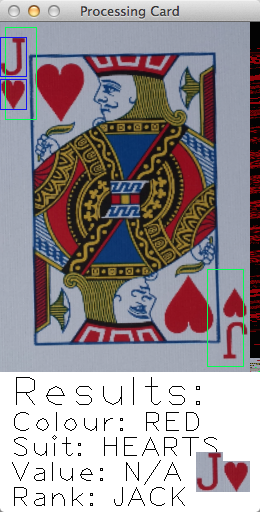
\includegraphics[width=0.4\textwidth]{symfind}
			\caption{An example of the results window of a single picture card image}
			\label{fig:symfind}
		\end{figure}

		These mats are only ever used for rank detection (J,Q,K,A), not value detection (2--10 inclusive) so there is no need to handle exceptional cases such as the fact that the value symbol `10' has two blobs instead of one. The isolated symbols can now be used for rank and suit classification.
	\counterwithin{figure}{subsubsection}
	\subsection{Value and Rank Detection}
		\label{sec:numdet}
				The rank of a card is determined by the numerical value in the top-left and bottom-right corners, and in the case of any card that is not a picture card, the quantity of suit symbols in the centre of the card itself. Thus, cards 2 through 10 are scored by their numerical value by the software implementation using the quantity of suit symbols.

		\subsubsection{Number cards}
			The first step in this classification stage is to convert the card image to a binary segmented form using simple thresholding, then by flood-filling the top-left and bottom-right corners, whose features are not used for value detection, as shown below:

			\begin{lstlisting}

cv::Mat temp = card->mat_bin.clone();

//Ignore the corners
cv::rectangle(temp, Card::TOP_CORNER_RECT, cv::Scalar(255), CV_FILLED);
cv::rectangle(temp, Card::BOTTOM_CORNER_RECT, cv::Scalar(255), CV_FILLED);
			\end{lstlisting}

			Once this is complete, the remaining blobs are morphologically eroded and closed to clear up the regions into single homogeneous blobs. This is done using custom morphological implementations which can be found in the source code under \source{cl\_own.cpp}{app:clowncpp}.

			\begin{lstlisting}

//Erode and close
temp = binary_operation(temp, MODE_BINARY_DILATION, 5);
temp = binary_closing(temp, 10);
			\end{lstlisting}

			The result is shown in Figure~\ref{fig:closing}:

			\begin{figure}[H]
				\centering
				\begin{subfigure}[b]{0.4\textwidth}
					\centering
					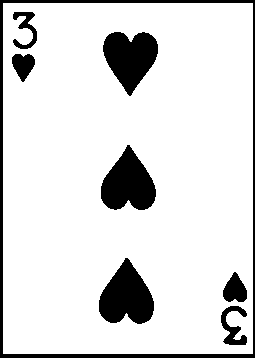
\includegraphics[width=\textwidth]{chris/image20}
					\caption{}
				\end{subfigure}
				\begin{subfigure}[b]{0.4\textwidth}
					\centering
					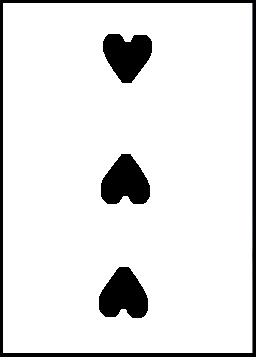
\includegraphics[width=\textwidth]{chris/image21}
					\caption{}
				\end{subfigure}
				\caption{Binary threshold segmented card with extraneous features removed}
				\label{fig:closing}
			\end{figure}

			After this, the remaining blobs are counted and filled, and is equal to the value of the card itself for the sample deck used for evaluation.

		\subsubsection{Picture cards}
			In the case of picture cards (except for the case of an Ace), there is to relationship between the number of blobs in the centre of the card and its value, such as a King. To get around this, the presence of a picture card is determined by the presence of an additional contour inside the isolated card, i.e.: there is a rectangle within the card rectangle, as illustrated below:

			\begin{figure}[H]
				\centering
				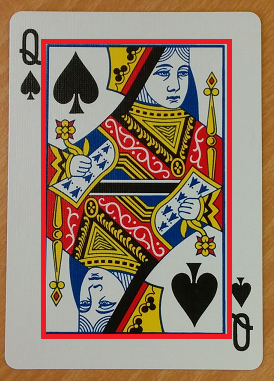
\includegraphics[width=0.4\textwidth]{chris/image22}
				\caption{A picture card such as Jack, Queen or King will have an interior contour}
				\label{fig:innercont}
			\end{figure}

			If this additional internal contour is found, its rank is determined using the rank symbol; `J', `Q' or `K', using a morphological Hit-or-Miss implementation. The region containing the isolated rank symbol area is used as the subject of a Hit-or-Miss pattern matching search against pre-created templates (or Structuring Elements), shown in Figure~\ref{fig:picstruct}:

			\begin{figure}[H]
				\centering
				\begin{subfigure}[b]{0.14\textwidth}
					\centering
					
\includegraphics[width=\textwidth]{chris/image23}
					\caption{}
				\end{subfigure}
				\begin{subfigure}[b]{0.15\textwidth}
					\centering
					
\includegraphics[width=\textwidth]{chris/image24}
					\caption{}
				\end{subfigure}
				\begin{subfigure}[b]{0.14\textwidth}
					\centering
					
\includegraphics[width=\textwidth]{chris/image25}
					\caption{}
				\end{subfigure}
				\caption{Pre-created Hit-or-Miss Structuring Elements for picture card rank evacuation}
				\label{fig:picstruct}
			\end{figure}

			When the pattern matching is carried out, both the isolated rank symbol area and the pre-created template are scaled to the same size before comparison. If the percentage of similar pixels exceeds a parametrised threshold, the card is classified to that rank. An example for the card shown in Figure~\ref{fig:queenstruct} is shown below:

			\begin{figure}[H]
				\centering
				\begin{subfigure}[b]{0.26\textwidth}
					\centering
					
\includegraphics[width=\textwidth]{chris/image26}
					\caption{}
				\end{subfigure}
				\begin{subfigure}[b]{0.25\textwidth}
					\centering
					
\includegraphics[width=\textwidth]{chris/image37}
					\caption{}
				\end{subfigure}
				\caption{Identically scaled isolated rank symbol (a) and template (b)}
				\label{fig:queenstruct}
			\end{figure}

			The percentage match between the three rank symbol templates shown in Figure~\ref{fig:picstruct} are output to the system console, and show a clear match for `Q' for the card in Figure~\ref{fig:innercont}:

			\begin{figure}[H]
				\centering
				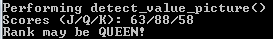
\includegraphics[width=0.6\textwidth]{chris/image27}
				\caption{Console output shows percentage match in clear favour of a Queen rank classification.}
				\label{fig:console}
			\end{figure}

			This entire process is shown in the implementation segment below (abbreviated):

			\begin{lstlisting}

//Load original SEs
cv::Mat se_symbols[3] = {
	cv::imread("res/symbols/scale_full/jack.png", CV_LOAD_IMAGE_GRAYSCALE),
	cv::imread("res/symbols/scale_full/queen.png", CV_LOAD_IMAGE_GRAYSCALE),
	cv::imread("res/symbols/scale_full/king.png", CV_LOAD_IMAGE_GRAYSCALE)
};

//Calculate new size
cv::Size size(100, 100);
cv::resize(mat_rank_1c, mat_rank_1c, size); //Should always be resized at runtime

//For reach symbol, resize SE
for(int j = 0; j < 3; j++)
{
	//Resize SE
	cv::resize(se_symbols[j], se_symbols[j], size); 
}

//Do matches using colour info integration
matches[JACK] += (int)round(hit_or_miss_score(mat_rank_1c, se_symbols[JACK]) * 100.0F);
matches[QUEEN] += (int)round(hit_or_miss_score(mat_rank_1c, se_symbols[QUEEN]) * 100.0F);
matches[KING] += (int)round(hit_or_miss_score(mat_rank_1c, se_symbols[KING]) * 100.0F);

cv::imshow("input", mat_rank_1c);
cv::imshow("template", se_symbols[QUEEN]);  //Only relevant for threecards.jpg

cout << "Scores (J/Q/K): " << matches[JACK] << "/" << matches[QUEEN] << "/" << matches[KING] << endl;

//Find which suit was matched most
if(max(matches[JACK], matches[QUEEN], matches[KING]) == matches[JACK])
{
	cout << "Rank may be JACK!" << endl;
	card->detected_rank = Card::RANK_JACK;
}
else if(max(matches[QUEEN], matches[QUEEN], matches[KING]) == matches[QUEEN])
{
	cout << "Rank may be QUEEN!" << endl;
	card->detected_rank = Card::RANK_QUEEN;
}
else if(max(matches[KING], matches[QUEEN], matches[KING]) == matches[KING])
{
	cout << "Rank may be KING!" << endl;
	card->detected_rank = Card::RANK_KING;
}
else
{
	cout << "No winner! UNKNOWN SUIT" << endl;
	card->detected_suit = Card::UNKNOWN_SUIT;
}
			\end{lstlisting}

		\subsubsection{Custom HoM Implementation}
			Mathematical Morphology operations are available as part of the OpenCV library (\code{cv::morphologyEx()}), but as a result of study of the theory and experimental requirements it was felt that a custom implementation of the theory was appropriate. This allows additional modification and parameterisation of the behaviour of required morphological operators. To this end the implementation uses the \code{binary_operation()}, \code{binary_closing()} and \code{hit_or_miss()} functions whose core workings are detailed below:

			A binary morphological erosion or dilation is performed on a pixel by pixel basis, with each pixel in the input image used as the centre of a symmetrical structuring element. In the case of erosion, the lowest value (any 0s) is set at the output pixel. In the case of dilation the greatest value (any 255s) is set as the output pixel. This is shown in the code segment below:

			\begin{lstlisting}

//For all X x Y pixels
int result = 0;
for(int y = 0; y < input.rows; y++)
{
	for(int x = 0; x < input.cols; x++)
	{
		//Reset for new neighbourhood
		result = 0;
			
		//Get local values
		bool break_now = false;
		for(int j = 0; j < element_size; j++)
		{
			for(int i = 0; i < element_size; i++)
			{
				//If in the image
				if(is_in_image((x - half) + i, (y - half) + j, input.cols, input.rows))
				{
					//Channel values
					int p = data[((y - half) + j) * input.step + ((x - half) + i) * input_channels];

					//Save brightest of that area
					if(mode == MODE_BINARY_DILATION)
					{
						if(p  > 128.0F) //Assuming binary input
						{
							result = 255;
							break_now = true;
							break;
						}
					}
					else
					{
						if(p < 128.0F)
						{
							result = 0;
							break_now = true;
							break;
						}
						else
						{
							result = 255;
						}
					}
				}
			}

			if(break_now == true)   //This is used for speed. Eg for erosion, if any are black, all become black
			{
				break;
			}
		}
	
		//Save output Mat data
		out_data[y * output.step + x * output_channels] = result;
	}
}
			\end{lstlisting}

			The end result of this operation is a \code{cv::Mat} containing an eroded or dilated image, depending on the mode passed as an argument. 

			The \code{binary_opening()} and \code{binary_closing()} functions simply chain calls to \code{binary_operation()} to implement the order of operations required for each operator. The example of \code{binary_closing()} is shown below:

			\begin{lstlisting}

cv::Mat binary_closing(cv::Mat input, int element_size)
{
	cout << "Performing binary closing..." << endl;

	cv::Mat working = input.clone();
	working = binary_operation(working, MODE_BINARY_DILATION, element_size);
	working = binary_operation(working, MODE_BINARY_EROSION, element_size);
	return working;
}
			\end{lstlisting}

			Finally, the morphological Hit-or-Miss transform is implemented by comparing all pixels in an input image to those in the equivalent locations in the structuring element image. Once all pixels have been compared, the total number of matched pixels is compared against a minimum to count as a match. In the case of \code{hit_or_miss_score()} the raw percentage of matched pixels is output as the return value. The implementation in code is shown below:

			\begin{lstlisting}

//For each position, try and find a match
int matched_pixels = 0;

//Search whole SE
for(int j = 0; j < img.rows; j++)
{
	for(int i = 0; i < img.cols; i++)
	{
		//Input pixel value
		int in_p = in_data[j * img.step + i * in_channels];
		int se_p = se_data[j * img.step + i * se_channels];

		//Minithresh - but should be binary anyway!
		in_p = in_p > 128 ? 255 : 0;
		se_p = se_p > 128 ? 255 : 0;

		if(in_p == se_p)
		{
			//Matching pixel found!
			matched_pixels++;
		}
	}
}

//Was this a matched template?
int total_pixels = img.rows * img.cols;
return (float)matched_pixels / (float)total_pixels;
			\end{lstlisting}

			This return value is then used to compare multiple structuring elements in the picture card rank finding as well as the suit symbol detection functions.
	\counterwithin{figure}{subsection}
	\subsection{Suit Symbol Detection}
				Once a card has been isolated from an image and its perspective correctly transformed, the isolated suit symbol in the top-left corner is compared to a set of pre-created symbols using the previously discussed Hit-or-Miss Transform.

		This operation is completed in two stages. First, the suit colour is determined, then the symbol is pattern matched. The suit search space is halved by the suit colour evaluation and also aids detection accuracy by defining pairs of suits as mutually exclusive in the detection. For example, a hearts symbol cannot be miss-classified as a spaces symbol once the colour of the suit is determined.

		\begin{figure}[H]
			\centering
			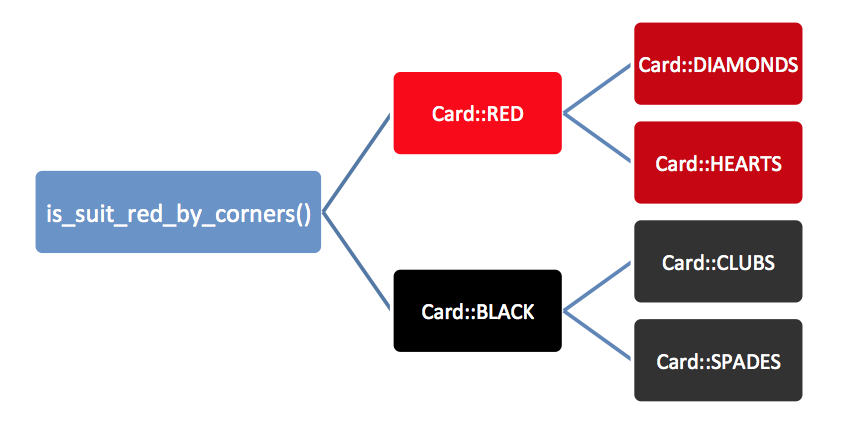
\includegraphics[width=0.95\textwidth]{chris/image38}
			\caption{Flow diagram of suit symbol classification showing mutually exclusive possibilities based on detected colour.}
		\end{figure}

		This decision is shown in the code segment below:

		\begin{lstlisting}

//Do matches using colour info integration
if(card->detected_colour == Card::RED)
{
	matches[DIAMOND] += (int)round(hit_or_miss_score(mat_sym_1c, se_symbols[DIAMOND]) * 100.0F);
	matches[HEART] += (int)round(hit_or_miss_score(mat_sym_1c, se_symbols[HEART]) * 100.0F);
}
else if(card->detected_colour == Card::BLACK)
{
	matches[CLUB] += (int)round(hit_or_miss_score(mat_sym_1c, se_symbols[CLUB]) * 100.0F);
	matches[SPADE] += (int)round(hit_or_miss_score(mat_sym_1c, se_symbols[SPADE]) * 100.0F);
}
else
{
	cout << "Colour has not been detected before find_suit_sym()!" << endl;
	return;
}
		\end{lstlisting}

		The second stage is performed with the Hit-or-Miss Transform applied to the isolated symbol \code{cv::Mat} using each of four pre-created symbol images, shown in Figure~\ref{fig:structelems}, after being resized to the same dimensions.

		\begin{figure}[H]
			\centering
			\begin{subfigure}[b]{0.15\textwidth}
				\centering
				
\includegraphics[width=\textwidth]{chris/image28}
				\caption{}
			\end{subfigure}
			\begin{subfigure}[b]{0.15\textwidth}
				\centering
				\includegraphics[width=\textwidth]{chris/image29}
				\caption{}
			\end{subfigure}
			\begin{subfigure}[b]{0.15\textwidth}
				\centering
				\includegraphics[width=\textwidth]{chris/image30}
				\caption{}
			\end{subfigure}
			\begin{subfigure}[b]{0.15\textwidth}
				\centering
				\includegraphics[width=\textwidth]{chris/image31}
				\caption{}
			\end{subfigure}
			\caption{The four pre-created suit symbol structuring elements.}
			\label{fig:structelems}
		\end{figure}

		Once both of the two applicable coloured structuring element images have been compared, the winning percentage match is then attributed in the structure for that card:

		\begin{lstlisting}

//Find which suit was matched most
if(max(matches[CLUB], matches[DIAMOND], matches[HEART], matches[SPADE]) == matches[CLUB])
{
	cout << "Suit may be CLUBS!" << endl;
	card->detected_suit = Card::CLUBS;  
}
else if(max(matches[CLUB], matches[DIAMOND], matches[HEART], matches[SPADE]) == matches[DIAMOND])
{
	cout << "Suit may be DIAMONDS!" << endl;
	card->detected_suit = Card::DIAMONDS;
}
else if(max(matches[CLUB], matches[DIAMOND], matches[HEART], matches[SPADE]) == matches[HEART])
{
	cout << "Suit may be HEARTS!" << endl;
	card->detected_suit = Card::HEARTS;
}
else if(max(matches[CLUB], matches[DIAMOND], matches[HEART], matches[SPADE]) == matches[SPADE])
{
	cout << "Suit may be SPADES!" << endl;
	card->detected_suit = Card::SPADES;
}
else
{
	cout << "No winner! UNKNOWN SUIT" << endl;
	card->detected_suit = Card::UNKNOWN_SUIT;
}
		\end{lstlisting}

		This matching is shown visually in the figure below in the case of a hearts card:

		\begin{figure}[H]
			\centering
			\includegraphics[width=0.6\textwidth]{chris/image32}
			\caption{Isolated and segmented card suit symbol and pre-created template used for comparison.}
		\end{figure}

		In this way the suit symbol is identified as contributes to the classification of the card in question.
	\subsection{Results Output}
		\label{sec:resultsout}
				Once all prior processes have been completed, the results of classification are output in two forms, as a GUI and on the system console. The GUI output is illustrated in the figure below:
		
		\begin{figure}[H]
			\centering
			\includegraphics[width=0.4\textwidth]{chris/image33}
			\caption{Card classification GUI output showing card isolated (a), isolated suit symbol (b), isolated rank symbol (c) and textual results output (d).}
		\end{figure}

		For each detected card in the input image, the classified suit colour, suit symbol, value (0 for picture cards) and the rank detected (N/A for number cards) are shown in their own view tile.
		
		In this method of output it is easy to determine which elements of classification have succeeded or why they have failed when they do. For example, the isolated suit and rank symbol image matrices are reproduced at the bottom of the window, and therefore in the event of a problem in classification the intermediary isolations can be checked for errors. 
		
		The second form of output is shown in the form of a natural language result in the system console. A string is concatenated using all the fields stored in the \code{Card} structure once classification is complete to form a single plain-English sentence. The code segment below illustrates how this is done:

		\begin{lstlisting}

//Nice CMD summary
cout << endl << "============== Detected Cards ==============" << endl << endl;

for(size_t i = 0; i < cards.size(); i++)
{
    cout << "Card " << (i + 1) << ": The ";

    if(cards[i].is_picture_card)
    {
        switch(cards[i].detected_rank)
        {
        case Card::RANK_JACK:
            cout << "Jack";
            break;
        case Card::RANK_QUEEN:
            cout << "Queen";
            break;
        case Card::RANK_KING:
            cout << "King";
            break;
        case Card::RANK_ACE:
            cout << "Ace";
            break;
        default:
            cout << "Something";
            break;
        }
    }
    else
    {
        cout << cards[i].detected_value;
    }

    cout << " of ";

    switch(cards[i].detected_suit)
    {
    case Card::CLUBS:
        cout << "Clubs";
        break;
    case Card::DIAMONDS:
        cout << "Diamonds";
        break;
    case Card::HEARTS:
        cout << "Hearts";
        break;
    case Card::SPADES:
        cout << "Spades";
        break;
    default:
        cout << "Something";
        break;
    }

    cout << endl;
}

cout << endl << "============================================" << endl << endl;
		\end{lstlisting}

		This is repeated for each card in the cascade, and is shown below for an example cascade of classified cards:

		\begin{figure}[H]
			\centering
			\begin{subfigure}[b]{\textwidth}
				\centering
				\includegraphics[width=\textwidth]{chris/image34}
				\caption{}
			\end{subfigure}
		\end{figure}
		\begin{figure}[H]
			\ContinuedFloat
			\centering
			\begin{subfigure}[b]{\textwidth}
				\centering
				\includegraphics[width=\textwidth]{chris/image35}
				\caption{}
			\end{subfigure}
			\caption{Example correct classification cascade of six cards showing GUI (a) and console output (b) formats.}
		\end{figure}

		A criterion for improvement for future expansion or interoperability of the software with other systems could be a CSV (comma separated values) output or network connectivity, both of which are not too difficult to implement.
	\counterwithin{figure}{subsubsection}
\pagebreak
\section{Evaluation}
	\counterwithin{figure}{section}
	Due to the nature of this system, evaluation is not very easy to do. In general, there are two high-level phases: card isolation and card classification. With isolation, there are so many possible scenarios and environments (one card, ten cards, fifty cards, partial occlusion, day, night, motion blur etc.) that it is impossible to test for all of them. Therefore, for the purpose of validation. A number of criteria were created.

	\begin{enumerate}
		\item Every card would be sampled at least four times where it is the only card in the image. The sample size per card is only four due to the fact that card appearance will not change across samples. Only images with single cards are processed due to the fact that the number of permutations is considerably large and would require disproportionate effort to perform for multiple cards.
		\item Every sample image is at a resolution of 640x480. Since it was already proven that multiple cards can be recognised, it is assumed that if a single card in a low resolution can be recognised, that the same card can be recognised in an image with multiple cards. 640x480 is a common resolution for cheap webcams. The resolution is fixed to not introduce discrepancies in processing speed/complexities.
		\item The background is matte green and the setting is a well-lit indoor room. This is to emulate the most realistic practical use case for this system; a casino table. A fixed webcam takes overhead images at a low resolution and at a low height to emulate a realistic scenario where a high resolution camera can be used to capture multiple cards from a high height above a poker table for instance.
		\item The minimum 4 samples for any card are captured with the card parallel to the camera, but at differing orientations. These are tilted to the left (e.g. Figure~\ref{fig:webcam}; zoom in if reading digitally), straightened, tilted to the right, and on its side (by 90 degrees). The other orientations are redundant due to a card's symmetry.
		\item If all four samples are classified correctly, it is assumed that the system will continue to do so for that card and is deemed valid. If the system misclassifies a card four samples in a row, then a total of eight samples are captured instead of four to make sure the misclassification was not a fluke and to increase the sample size somewhat for added accuracy.
		\item In addition, the system is run on a blank background to test the ability to detect that there are no cards.
	\end{enumerate}

	\begin{figure}[H]
		\centering
		\includegraphics[width=0.06\linewidth]{webcam/img0}
		\includegraphics[width=0.06\linewidth]{webcam/img1}
		\includegraphics[width=0.06\linewidth]{webcam/img2}
		\includegraphics[width=0.06\linewidth]{webcam/img3}
		\includegraphics[width=0.06\linewidth]{webcam/img4}
		\includegraphics[width=0.06\linewidth]{webcam/img5}
		\includegraphics[width=0.06\linewidth]{webcam/img6}
		\includegraphics[width=0.06\linewidth]{webcam/img7}
		\includegraphics[width=0.06\linewidth]{webcam/img8}
		\includegraphics[width=0.06\linewidth]{webcam/img9}
		\includegraphics[width=0.06\linewidth]{webcam/img10}
		\includegraphics[width=0.06\linewidth]{webcam/img11}
		\includegraphics[width=0.06\linewidth]{webcam/img12}\\[3px]
		\includegraphics[width=0.06\linewidth]{webcam/img13}
		\includegraphics[width=0.06\linewidth]{webcam/img14}
		\includegraphics[width=0.06\linewidth]{webcam/img15}
		\includegraphics[width=0.06\linewidth]{webcam/img16}
		\includegraphics[width=0.06\linewidth]{webcam/img17}
		\includegraphics[width=0.06\linewidth]{webcam/img18}
		\includegraphics[width=0.06\linewidth]{webcam/img19}
		\includegraphics[width=0.06\linewidth]{webcam/img20}
		\includegraphics[width=0.06\linewidth]{webcam/img21}
		\includegraphics[width=0.06\linewidth]{webcam/img22}
		\includegraphics[width=0.06\linewidth]{webcam/img23}
		\includegraphics[width=0.06\linewidth]{webcam/img24}
		\includegraphics[width=0.06\linewidth]{webcam/img25}\\[3px]
		\includegraphics[width=0.06\linewidth]{webcam/img26}
		\includegraphics[width=0.06\linewidth]{webcam/img27}
		\includegraphics[width=0.06\linewidth]{webcam/img28}
		\includegraphics[width=0.06\linewidth]{webcam/img29}
		\includegraphics[width=0.06\linewidth]{webcam/img30}
		\includegraphics[width=0.06\linewidth]{webcam/img31}
		\includegraphics[width=0.06\linewidth]{webcam/img32}
		\includegraphics[width=0.06\linewidth]{webcam/img33}
		\includegraphics[width=0.06\linewidth]{webcam/img34}
		\includegraphics[width=0.06\linewidth]{webcam/img35}
		\includegraphics[width=0.06\linewidth]{webcam/img36}
		\includegraphics[width=0.06\linewidth]{webcam/img37}
		\includegraphics[width=0.06\linewidth]{webcam/img38}\\[3px]
		\includegraphics[width=0.06\linewidth]{webcam/img39}
		\includegraphics[width=0.06\linewidth]{webcam/img40}
		\includegraphics[width=0.06\linewidth]{webcam/img41}
		\includegraphics[width=0.06\linewidth]{webcam/img42}
		\includegraphics[width=0.06\linewidth]{webcam/img43}
		\includegraphics[width=0.06\linewidth]{webcam/img44}
		\includegraphics[width=0.06\linewidth]{webcam/img45}
		\includegraphics[width=0.06\linewidth]{webcam/img46}
		\includegraphics[width=0.06\linewidth]{webcam/img47}
		\includegraphics[width=0.06\linewidth]{webcam/img48}
		\includegraphics[width=0.06\linewidth]{webcam/img49}
		\includegraphics[width=0.06\linewidth]{webcam/img50}
		\includegraphics[width=0.06\linewidth]{webcam/img51}\\[3px]
		\caption{An example of canonical webcam samples at a single orientation}
		\label{fig:webcam}
	\end{figure}

	With webcam tests and a sample size of 232 images of single cards, card finding succeeded 99.14\% of the time. When it failed, it was on the inner contours of a picture card. Remedies to this are discussed in the further improvements section \secref{sec:improvements}. For card classification confusion matrices are constructed (NB: All confusion matrices have actual classes as rows and predicted classes as columns). The first is one for every single card (52x52 elements). Due to the fact that it is (fortunately) mostly zeroes and that mostly the diagonals contain the full count of samples, the working classes are culled and only the interesting parts are presented for the purpose of this report in Table~\ref{tab:genconf} on page~\pageref{tab:genconf}.

	Additionally a smaller confusion matrix for just suits can be constructed with sample sizes that allow a much more accurate evaluation of performance:

	\begin{table}[H]
		\centering
		\caption{The suit confusion matrix}
		\label{tab:suitconf}
		\begin{tabular}{| l || l | l | l | l || l |}
			\hline
			         & Spades & Hearts & Diamonds & Clubs & Accuracies\\
			\hhline{|=|=|=|=|=|=|}
			Spades   & 59\cellcolor[gray]{0.9}  & 0  & 0  & 1\cellcolor[gray]{0.9}  & 93.31\% \\
			\hline
			Hearts   & 0  & 52\cellcolor[gray]{0.9}  & 8\cellcolor[gray]{0.9}  & 0  & 84.63\% \\
			\hline
			Diamonds & 0  & 0  & 52\cellcolor[gray]{0.9}  & 0  & 100\% \\
			\hline
			Clubs    & 0  & 0 & 0  & 52\cellcolor[gray]{0.9}  & 100\% \\
			\hline
		\end{tabular}
	\end{table}

	Notice how colour classification accuracy is at 100\%. Suit accuracy however is not perfect. This data shows that diamonds are always classified as diamonds but some hearts are also classified as diamonds; diamond classification is too aggressive. The same goes for clubs with respect to spades. This would become more clear if the rows and columns in Table~\ref{tab:genconf} were sorted by suit first, then value/rank. That table shows however that type detection (i.e. numbers vs. picture cards) accuracy is at 96.55\%.

	Overall system accuracy is at 93\%. While this is not spectacular, bear in mind the small sample sizes per card due to the nature of this system. If for example the sample size was four and 1/4 was classified incorrectly by some fluke or random chance occurrence, already that is a performance of 75\%. With a sample size of 100 per card for instance, the same fluke would be reduced to 1/100 --- or a performance of 99\%.

	Furthermore, 50/52 (96.2\%) of the cards could be successfully identified. The ones that could not were the Ace of Spades --- due to the complex motif in its centre which the system did not have a contingency for --- and the 7 of hearts which had its orientation incorrectly rotated due to one of the heart symbols encroaching in on corner space and confusing the whiteness measure function discussed earlier. Clearly there is some room for improvement under the circumstances, yet all things considered, the system works quite splendidly.

	\pagebreak
	\begin{landscape}
		\begin{table}[t]
			\centering
			\caption{The abridged general confusion matrix}
			\label{tab:genconf}
			\begin{tabular}{| l || l | l | l | l | l | l | l | l | l | l | l | l | l | l | l || l | l |}
				\hline
				            & AS & 4S & 7H & 7D & 8D & 9D & 10D & JS & JH & JD & JC & QD & KD & N/A & All Others & Sample Size & Accuracies \\
				\hhline{|=|=|=|=|=|=|=|=|=|=|=|=|=|=|=|=|=|=|}
				AS          & 0  & 8\cellcolor[gray]{0.9}  & 0  & 0  & 0  & 0  & 0   & 0  & 0  & 0  & 0  & 0  & 0  & 0   & 0          & 8           &    0\%     \\
				\hline
				7H          & 0  & 0  & 0  & 0  & 4\cellcolor[gray]{0.9}  & 2\cellcolor[gray]{0.9}  & 0   & 0  & 0  & 0  & 0  & 2\cellcolor[gray]{0.9}  & 0  & 0   & 0          & 8           &    0\%     \\
				\hline
				7D          & 0  & 0  & 0  & 3\cellcolor[gray]{0.9}  & 0  & 0  & 0   & 0  & 0  & 1\cellcolor[gray]{0.9}  & 0  & 0  & 0  & 0   & 0          & 4           &   75\%     \\
				\hline
				9D          & 0  & 0  & 0  & 0  & 0  & 3\cellcolor[gray]{0.9}  & 0   & 0  & 0  & 1\cellcolor[gray]{0.9}  & 0  & 0  & 0  & 0   & 0          & 4           &   75\%     \\
				\hline
				JS          & 0  & 0  & 0  & 0  & 0  & 0  & 0   & 4\cellcolor[gray]{0.9}  & 0  & 0  & 1\cellcolor[gray]{0.9}  & 0  & 0  & 3\cellcolor[gray]{0.9}   & 0          & 8           &   50\%     \\
				\hline
				JH          & 0  & 0  & 0  & 0  & 0  & 0  & 0   & 0  & 3\cellcolor[gray]{0.9}  & 0  & 0  & 0  & 0  & 5\cellcolor[gray]{0.9}   & 0          & 8           & 37.5\%     \\
				\hline
				KD          & 0  & 0  & 0  & 0  & 3\cellcolor[gray]{0.9}  & 0  & 1\cellcolor[gray]{0.9}   & 0  & 0  & 0  & 0  & 0  & 4\cellcolor[gray]{0.9}  & 0   & 0          & 8           &   50\%     \\
				\hline
				All Others  & 0  & 0  & 0  & 0  & 0  & 0  & 0   & 0  & 0  & 0  & 0  & 0  & 0  & 0   & 0          & 4           &  100\%     \\
				\hline
			\end{tabular}
		\end{table}
	\end{landscape}
	\pagebreak
	\counterwithin{figure}{subsubsection}
\pagebreak
\section{Conclusion}
	\subsection{Summary}
		After completing this assignment, an greater understanding has been obtained into the current fields of computer vision and mathematical morphology. Techniques such as CLAHE, Hough Transform and morphological operations such as erosion, closing and the Hit-or-Miss Transform have been found favourable for the assignment task of automated classification of playing cards.

		This has been translated into a C++ software solution overcoming obstacles such as invalid cards, various orientations (through perspective transform operations) and variable lighting. Images can contain multiple cards and can be sourced from a local directory or captured live from a webcam through the use of a simple command line flag.

		Evaluation of the software has been performed by a structured progression from synthetic images through to real images of single cards, multiple cards per scene and finally accuracy measurement through use of a confusion matrix to identify miss-classifications.
	\subsection{Improvements}
		\label{sec:improvements}
		Due to time limitation, the software was developed to work well with the most commonly encountered classic playing card style. Therefore the main weakness is that any kind of themed or differently stylized decks of cards will not result in the same level of performance. Other possible improvements include:
		\begin{itemize}
			\item Improving the pre-processing and equalisation to reduce incorrectly identified card contours and better cope with more extreme lighting conditions.
			\item Use a thread based approach (requires C++11 compilation, currently unused) to concurrently perform pattern matching and other time consuming processes to reduce time between image capture and classification output. More sample sizes can increase detection accuracy, as well as possible orientation matching to utilise the suit symbol in the lower right corner of the card to improve accuracy.
			\item Implement more data interfaces such as output to a CSV file, integration with a TCP connection for remote monitoring and processing, or to a connected microcontroller for more immediate environment interaction. 
			\item The possibility of implementation on a GPU proper using CUDA or OpenCL could be explored, allowing much faster classification.
		\end{itemize}
\pagebreak
\thispagestyle{empty}
\printbibliography
\pagebreak
\begin{appendices}
	\section{Contribution Agreement}
		\begin{figure}[H]
			\centering
			\includegraphics[width=\textwidth]{chris/image36}
		\end{figure}
		Report contributions by section are 1, 2.1.2, 3.1, 4.1, 4.2, 4.4, 4.7, 4.8, 4.9 and 6 for Chris and 2.1.1, 4.3, 4.5, 4.6, and 5 for Yousef. Each member generally wrote about the parts of the project they were involved with. Git was used for collaboration and version control.
	\pagebreak
	\section{Fully Documented Source Code Listings}
		\lstset{
			language=C++,
			showspaces=false,
			showtabs=false,
			breaklines=true,
			breakatwhitespace=true,
			escapeinside={(*@}{@*)},
			commentstyle=\color{greencomments},
			keywordstyle=\color{bluekeywords},
			stringstyle=\color{redstrings},
			basicstyle=\ttfamily\scriptsize,
			captionpos=t,
			extendedchars=true,
			frame=single,
			keepspaces=true,
			showstringspaces=false,
			stepnumber=2,
			tabsize=2,
		}
		\subsection{main.cpp}
		\label{app:maincpp}
		\lstinputlisting{res/appendices/src/main.cpp}
		\subsection{stdafx.h}
		\lstinputlisting{res/appendices/include/stdafx.h}
		\subsection{stdafx.cpp}
		\lstinputlisting{res/appendices/src/stdafx.cpp}
		\subsection{card.h}
		\lstinputlisting{res/appendices/include/card.h}
		\subsection{card.cpp}
		\lstinputlisting{res/appendices/src/card.cpp}
		\subsection{preprocessing.h}
		\lstinputlisting{res/appendices/include/preprocessing.h}
		\subsection{preprocessing.cpp}
		\lstinputlisting{res/appendices/src/preprocessing.cpp}
		\subsection{isolation.h}
		\lstinputlisting{res/appendices/include/isolation.h}
		\subsection{isolation.cpp}
		\label{app:isolationcpp}
		\lstinputlisting{res/appendices/src/isolation.cpp}
		\subsection{cl\_own.h}
		\lstinputlisting{res/appendices/include/cl_own.h}
		\subsection{cl\_own.cpp}
		\label{app:clowncpp}
		\lstinputlisting{res/appendices/src/cl_own.cpp}
		\subsection{classification.h}
		\lstinputlisting{res/appendices/include/classification.h}
		\subsection{classification.cpp}
		\label{app:classificationcpp}
		\lstinputlisting{res/appendices/src/classification.cpp}
		\subsection{utils.h}
		\lstinputlisting{res/appendices/include/utils.h}
		\subsection{utils.cpp}
		\lstinputlisting{res/appendices/src/utils.cpp}
\end{appendices}

\vfill
\hrulefill

\end{document}